%

%% bare_jrnl.tex
%% V1.3
%% 2007/01/11
%% by Michael Shell
%% see http://www.michaelshell.org/
%% for current contact information.
%%
%% This is a skeleton file demonstrating the use of IEEEtran.cls
%% (requires IEEEtran.cls version 1.7 or later) with an IEEE journal paper.
%%
%% Support sites:
%% http://www.michaelshell.org/tex/ieeetran/
%% http://www.ctan.org/tex-archive/macros/latex/contrib/IEEEtran/
%% and
%% http://www.ieee.org/



% *** Authors should verify (and, if needed, correct) their LaTeX system  ***
% *** with the testflow diagnostic prior to trusting their LaTeX platform ***
% *** with production work. IEEE's font choices can trigger bugs that do  ***
% *** not appear when using other class files.                            ***
% The testflow support page is at:
% http://www.michaelshell.org/tex/testflow/


%%*************************************************************************
%% Legal Notice:
%% This code is offered as-is without any warranty either expressed or
%% implied; without even the implied warranty of MERCHANTABILITY or
%% FITNESS FOR A PARTICULAR PURPOSE! 
%% User assumes all risk.
%% In no event shall IEEE or any contributor to this code be liable for
%% any damages or losses, including, but not limited to, incidental,
%% consequential, or any other damages, resulting from the use or misuse
%% of any information contained here.
%%
%% All comments are the opinions of their respective authors and are not
%% necessarily endorsed by the IEEE.
%%
%% This work is distributed under the LaTeX Project Public License (LPPL)
%% ( http://www.latex-project.org/ ) version 1.3, and may be freely used,
%% distributed and modified. A copy of the LPPL, version 1.3, is included
%% in the base LaTeX documentation of all distributions of LaTeX released
%% 2003/12/01 or later.
%% Retain all contribution notices and credits.
%% ** Modified files should be clearly indicated as such, including  **
%% ** renaming them and changing author support contact information. **
%%
%% File list of work: IEEEtran.cls, IEEEtran_HOWTO.pdf, bare_adv.tex,
%%                    bare_conf.tex, bare_jrnl.tex, bare_jrnl_compsoc.tex
%%*************************************************************************

% Note that the a4paper option is mainly intended so that authors in
% countries using A4 can easily print to A4 and see how their papers will
% look in print - the typesetting of the document will not typically be
% affected with changes in paper size (but the bottom and side margins will).
% Use the testflow package mentioned above to verify correct handling of
% both paper sizes by the user's LaTeX system.
%
% Also note that the "draftcls" or "draftclsnofoot", not "draft", option
% should be used if it is desired that the figures are to be displayed in
% draft mode.
%
\documentclass[journal]{IEEEtran}
%
% If IEEEtran.cls has not been installed into the LaTeX system files,
% manually specify the path to it like:
% \documentclass[journal]{../sty/IEEEtran}



% Some very useful LaTeX packages include:
% (uncomment the ones you want to load)


% *** MISC UTILITY PACKAGES ***
%
%\usepackage{ifpdf}
% Heiko Oberdiek's ifpdf.sty is very useful if you need conditional
% compilation based on whether the output is pdf or dvi.
% usage:
% \ifpdf
%   % pdf code
% \else
%   % dvi code
% \fi
% The latest version of ifpdf.sty can be obtained from:
% http://www.ctan.org/tex-archive/macros/latex/contrib/oberdiek/
% Also, note that IEEEtran.cls V1.7 and later provides a builtin
% \ifCLASSINFOpdf conditional that works the same way.
% When switching from latex to pdflatex and vice-versa, the compiler may
% have to be run twice to clear warning/error messages.






% *** CITATION PACKAGES ***
%
%\usepackage{cite}
% cite.sty was written by Donald Arseneau
% V1.6 and later of IEEEtran pre-defines the format of the cite.sty package
% \cite{} output to follow that of IEEE. Loading the cite package will
% result in citation numbers being automatically sorted and properly
% "compressed/ranged". e.g., [1], [9], [2], [7], [5], [6] without using
% cite.sty will become [1], [2], [5]--[7], [9] using cite.sty. cite.sty's
% \cite will automatically add leading space, if needed. Use cite.sty's
% noadjust option (cite.sty V3.8 and later) if you want to turn this off.
% cite.sty is already installed on most LaTeX systems. Be sure and use
% version 4.0 (2003-05-27) and later if using hyperref.sty. cite.sty does
% not currently provide for hyperlinked citations.
% The latest version can be obtained at:
% http://www.ctan.org/tex-archive/macros/latex/contrib/cite/
% The documentation is contained in the cite.sty file itself.


%\usepackage[numbered,framed]{matlab-prettifier}
%\usepackage{color}
\usepackage[usenames,dvipsnames,svgnames,table]{xcolor}
\usepackage{listings}



% *** GRAPHICS RELATED PACKAGES ***
\usepackage{ifpdf}
%\usepackage{paralist}
%\usepackage{amsfonts}
 \usepackage{subfig}
%\usepackage{subcaption}
\usepackage[pdftex]{graphicx}
  \usepackage{epstopdf}
   \ifpdf
  \usepackage[pdftex]{graphicx}
  \graphicspath{figures/}
  \DeclareGraphicsExtensions{.pdf,.jep,.png,.jpg}
 \else
  \usepackage[dvips]{graphicx}
  \graphicspath{figures/}
  \DeclareGraphicsExtensions{.eps}
 \fi



%
\ifCLASSINFOpdf
  % \usepackage[pdftex]{graphicx}
  % declare the path(s) where your graphic files are
  % \graphicspath{{../pdf/}{../jpeg/}}
  % and their extensions so you won't have to specify these with
  % every instance of \includegraphics
  % \DeclareGraphicsExtensions{.pdf,.jpeg,.png}
\else
  % or other class option (dvipsone, dvipdf, if not using dvips). graphicx
  % will default to the driver specified in the system graphics.cfg if no
  % driver is specified.
  % \usepackage[dvips]{graphicx}
  % declare the path(s) where your graphic files are
  % \graphicspath{{../eps/}}
  % and their extensions so you won't have to specify these with
  % every instance of \includegraphics
  % \DeclareGraphicsExtensions{.eps}
\fi
% graphicx was written by David Carlisle and Sebastian Rahtz. It is
% required if you want graphics, photos, etc. graphicx.sty is already
% installed on most LaTeX systems. The latest version and documentation can
% be obtained at: 
% http://www.ctan.org/tex-archive/macros/latex/required/graphics/
% Another good source of documentation is "Using Imported Graphics in
% LaTeX2e" by Keith Reckdahl which can be found as epslatex.ps or
% epslatex.pdf at: http://www.ctan.org/tex-archive/info/
%
% latex, and pdflatex in dvi mode, support graphics in encapsulated
% postscript (.eps) format. pdflatex in pdf mode supports graphics
% in .pdf, .jpeg, .png and .mps (metapost) formats. Users should ensure
% that all non-photo figures use a vector format (.eps, .pdf, .mps) and
% not a bitmapped formats (.jpeg, .png). IEEE frowns on bitmapped formats
% which can result in "jaggedy"/blurry rendering of lines and letters as
% well as large increases in file sizes.
%
% You can find documentation about the pdfTeX application at:
% http://www.tug.org/applications/pdftex





% *** MATH PACKAGES ***
%
\usepackage[cmex10]{amsmath}
% A popular package from the American Mathematical Society that provides
% many useful and powerful commands for dealing with mathematics. If using
% it, be sure to load this package with the cmex10 option to ensure that
% only type 1 fonts will utilized at all point sizes. Without this option,
% it is possible that some math symbols, particularly those within
% footnotes, will be rendered in bitmap form which will result in a
% document that can not be IEEE Xplore compliant!
%
% Also, note that the amsmath package sets \interdisplaylinepenalty to 10000
% thus preventing page breaks from occurring within multiline equations. Use:
%\interdisplaylinepenalty=2500
% after loading amsmath to restore such page breaks as IEEEtran.cls normally
% does. amsmath.sty is already installed on most LaTeX systems. The latest
% version and documentation can be obtained at:
% http://www.ctan.org/tex-archive/macros/latex/required/amslatex/math/





% *** SPECIALIZED LIST PACKAGES ***
%
\usepackage{algorithmic}
% algorithmic.sty was written by Peter Williams and Rogerio Brito.
% This package provides an algorithmic environment fo describing algorithms.
% You can use the algorithmic environment in-text or within a figure
% environment to provide for a floating algorithm. Do NOT use the algorithm
% floating environment provided by algorithm.sty (by the same authors) or
% algorithm2e.sty (by Christophe Fiorio) as IEEE does not use dedicated
% algorithm float types and packages that provide these will not provide
% correct IEEE style captions. The latest version and documentation of
% algorithmic.sty can be obtained at:
% http://www.ctan.org/tex-archive/macros/latex/contrib/algorithms/
% There is also a support site at:
% http://algorithms.berlios.de/index.html
% Also of interest may be the (relatively newer and more customizable)
% algorithmicx.sty package by Szasz Janos:
% http://www.ctan.org/tex-archive/macros/latex/contrib/algorithmicx/




% *** ALIGNMENT PACKAGES ***
%
\usepackage{array}
% Frank Mittelbach's and David Carlisle's array.sty patches and improves
% the standard LaTeX2e array and tabular environments to provide better
% appearance and additional user controls. As the default LaTeX2e table
% generation code is lacking to the point of almost being broken with
% respect to the quality of the end results, all users are strongly
% advised to use an enhanced (at the very least that provided by array.sty)
% set of table tools. array.sty is already installed on most systems. The
% latest version and documentation can be obtained at:
% http://www.ctan.org/tex-archive/macros/latex/required/tools/


%\usepackage{mdwmath}
%\usepackage{mdwtab}
% Also highly recommended is Mark Wooding's extremely powerful MDW tools,
% especially mdwmath.sty and mdwtab.sty which are used to format equations
% and tables, respectively. The MDWtools set is already installed on most
% LaTeX systems. The lastest version and documentation is available at:
% http://www.ctan.org/tex-archive/macros/latex/contrib/mdwtools/


% IEEEtran contains the IEEEeqnarray family of commands that can be used to
% generate multiline equations as well as matrices, tables, etc., of high
% quality.


%\usepackage{eqparbox}
% Also of notable interest is Scott Pakin's eqparbox package for creating
% (automatically sized) equal width boxes - aka "natural width parboxes".
% Available at:
% http://www.ctan.org/tex-archive/macros/latex/contrib/eqparbox/





% *** SUBFIGURE PACKAGES ***
%\usepackage[tight,footnotesize]{subfigure}
% subfigure.sty was written by Steven Douglas Cochran. This package makes it
% easy to put subfigures in your figures. e.g., "Figure 1a and 1b". For IEEE
% work, it is a good idea to load it with the tight package option to reduce
% the amount of white space around the subfigures. subfigure.sty is already
% installed on most LaTeX systems. The latest version and documentation can
% be obtained at:
% http://www.ctan.org/tex-archive/obsolete/macros/latex/contrib/subfigure/
% subfigure.sty has been superceeded by subfig.sty.



%\usepackage[caption=false]{caption}
%\usepackage[font=footnotesize]{subfig}
% subfig.sty, also written by Steven Douglas Cochran, is the modern
% replacement for subfigure.sty. However, subfig.sty requires and
% automatically loads Axel Sommerfeldt's caption.sty which will override
% IEEEtran.cls handling of captions and this will result in nonIEEE style
% figure/table captions. To prevent this problem, be sure and preload
% caption.sty with its "caption=false" package option. This is will preserve
% IEEEtran.cls handing of captions. Version 1.3 (2005/06/28) and later 
% (recommended due to many improvements over 1.2) of subfig.sty supports
% the caption=false option directly:
%\usepackage[caption=false,font=footnotesize]{subfig}
%
% The latest version and documentation can be obtained at:
% http://www.ctan.org/tex-archive/macros/latex/contrib/subfig/
% The latest version and documentation of caption.sty can be obtained at:
% http://www.ctan.org/tex-archive/macros/latex/contrib/caption/




% *** FLOAT PACKAGES ***
%
%\usepackage{fixltx2e}
% fixltx2e, the successor to the earlier fix2col.sty, was written by
% Frank Mittelbach and David Carlisle. This package corrects a few problems
% in the LaTeX2e kernel, the most notable of which is that in current
% LaTeX2e releases, the ordering of single and double column floats is not
% guaranteed to be preserved. Thus, an unpatched LaTeX2e can allow a
% single column figure to be placed prior to an earlier double column
% figure. The latest version and documentation can be found at:
% http://www.ctan.org/tex-archive/macros/latex/base/



%\usepackage{stfloats}
% stfloats.sty was written by Sigitas Tolusis. This package gives LaTeX2e
% the ability to do double column floats at the bottom of the page as well
% as the top. (e.g., "\begin{figure*}[!b]" is not normally possible in
% LaTeX2e). It also provides a command:
%\fnbelowfloat
% to enable the placement of footnotes below bottom floats (the standard
% LaTeX2e kernel puts them above bottom floats). This is an invasive package
% which rewrites many portions of the LaTeX2e float routines. It may not work
% with other packages that modify the LaTeX2e float routines. The latest
% version and documentation can be obtained at:
% http://www.ctan.org/tex-archive/macros/latex/contrib/sttools/
% Documentation is contained in the stfloats.sty comments as well as in the
% presfull.pdf file. Do not use the stfloats baselinefloat ability as IEEE
% does not allow \baselineskip to stretch. Authors submitting work to the
% IEEE should note that IEEE rarely uses double column equations and
% that authors should try to avoid such use. Do not be tempted to use the
% cuted.sty or midfloat.sty packages (also by Sigitas Tolusis) as IEEE does
% not format its papers in such ways.


%\ifCLASSOPTIONcaptionsoff
%  \usepackage[nomarkers]{endfloat}
% \let\MYoriglatexcaption\caption
% \renewcommand{\caption}[2][\relax]{\MYoriglatexcaption[#2]{#2}}
%\fi
% endfloat.sty was written by James Darrell McCauley and Jeff Goldberg.
% This package may be useful when used in conjunction with IEEEtran.cls'
% captionsoff option. Some IEEE journals/societies require that submissions
% have lists of figures/tables at the end of the paper and that
% figures/tables without any captions are placed on a page by themselves at
% the end of the document. If needed, the draftcls IEEEtran class option or
% \CLASSINPUTbaselinestretch interface can be used to increase the line
% spacing as well. Be sure and use the nomarkers option of endfloat to
% prevent endfloat from "marking" where the figures would have been placed
% in the text. The two hack lines of code above are a slight modification of
% that suggested by in the endfloat docs (section 8.3.1) to ensure that
% the full captions always appear in the list of figures/tables - even if
% the user used the short optional argument of \caption[]{}.
% IEEE papers do not typically make use of \caption[]'s optional argument,
% so this should not be an issue. A similar trick can be used to disable
% captions of packages such as subfig.sty that lack options to turn off
% the subcaptions:
% For subfig.sty:
% \let\MYorigsubfloat\subfloat
% \renewcommand{\subfloat}[2][\relax]{\MYorigsubfloat[]{#2}}
% For subfigure.sty:
% \let\MYorigsubfigure\subfigure
% \renewcommand{\subfigure}[2][\relax]{\MYorigsubfigure[]{#2}}
% However, the above trick will not work if both optional arguments of
% the \subfloat/subfig command are used. Furthermore, there needs to be a
% description of each subfigure *somewhere* and endfloat does not add
% subfigure captions to its list of figures. Thus, the best approach is to
% avoid the use of subfigure captions (many IEEE journals avoid them anyway)
% and instead reference/explain all the subfigures within the main caption.
% The latest version of endfloat.sty and its documentation can obtained at:
% http://www.ctan.org/tex-archive/macros/latex/contrib/endfloat/
%
% The IEEEtran \ifCLASSOPTIONcaptionsoff conditional can also be used
% later in the document, say, to conditionally put the References on a 
% page by themselves.





% *** PDF, URL AND HYPERLINK PACKAGES ***
%
%\usepackage{url}
% url.sty was written by Donald Arseneau. It provides better support for
% handling and breaking URLs. url.sty is already installed on most LaTeX
% systems. The latest version can be obtained at:
% http://www.ctan.org/tex-archive/macros/latex/contrib/misc/
% Read the url.sty source comments for usage information. Basically,
% \url{my_url_here}.





% *** Do not adjust lengths that control margins, column widths, etc. ***
% *** Do not use packages that alter fonts (such as pslatex).         ***
% There should be no need to do such things with IEEEtran.cls V1.6 and later.
% (Unless specifically asked to do so by the journal or conference you plan
% to submit to, of course. )


% correct bad hyphenation here
\hyphenation{op-tical net-works semi-conduc-tor}

\usepackage{hyperref}

\begin{document}

%
% paper title
% can use linebreaks \\ within to get better formatting as desired
\title{3D Tracking of Facial Features}
%
%
% author names and IEEE memberships
% note positions of commas and nonbreaking spaces ( ~ ) LaTeX will not break
% a structure at a ~ so this keeps an author's name from being broken across
% two lines.
% use \thanks{} to gain access to the first footnote area
% a separate \thanks must be used for each paragraph as LaTeX2e's \thanks
% was not built to handle multiple paragraphs
%

\author{Ayham Alharbat,~\IEEEmembership{a.alharbat@student.utwente.nl,~2379589,~MSc EE-RAM}
        
        ~Jeroen Ritmeester,~\IEEEmembership{email address,~student id,~educational program}% <-this % stops a space
		
		~Protik Banerji,~\IEEEmembership{p.banerji@student.utwente.nl,s2342898,Msc S&C-RAM}% <-this % stops a space
}

% note the % following the last \IEEEmembership and also \thanks - 
% these prevent an unwanted space from occurring between the last author name
% and the end of the author line. i.e., if you had this:
% 
% \author{....lastname \thanks{...} \thanks{...} }
%                     ^------------^------------^----Do not want these spaces!
%
% a space would be appended to the last name and could cause every name on that
% line to be shifted left slightly. This is one of those "LaTeX things". For
% instance, "\textbf{A} \textbf{B}" will typeset as "A B" not "AB". To get
% "AB" then you have to do: "\textbf{A}\textbf{B}"
% \thanks is no different in this regard, so shield the last } of each \thanks
% that ends a line with a % and do not let a space in before the next \thanks.
% Spaces after \IEEEmembership other than the last one are OK (and needed) as
% you are supposed to have spaces between the names. For what it is worth,
% this is a minor point as most people would not even notice if the said evil
% space somehow managed to creep in.



% The paper headers
\markboth{12-04-2020, Image Processing and Computer Vision}%
{Shell \MakeLowercase{\textit{et al.}}: Bare Demo of IEEEtran.cls for Journals}
% The only time the second header will appear is for the odd numbered pages
% after the title page when using the twoside option.
% 
% *** Note that you probably will NOT want to include the author's ***
% *** name in the headers of peer review papers.                   ***
% You can use \ifCLASSOPTIONpeerreview for conditional compilation here if
% you desire.




% If you want to put a publisher's ID mark on the page you can do it like
% this:
%\IEEEpubid{0000--0000/00\$00.00~\copyright~2007 IEEE}
% Remember, if you use this you must call \IEEEpubidadjcol in the second
% column for its text to clear the IEEEpubid mark.



% use for special paper notices
%\IEEEspecialpapernotice{(Invited Paper)}




% make the title area
\maketitle


\begin{abstract}
%\boldmath
In this paper, a 3D facial features tracking system is developed to track facial features and measure the mobility of the tongue tip. The system uses Kanade-Lucas-Tomasi tracking algorithm to track a set of points of interest, and it uses Random Sample Consensus algorithm to eliminate the outliers and estimate parameters. Then these parameters are used to measure the tracked points in 3D space.
\end{abstract}
% IEEEtran.cls defaults to using nonbold math in the Abstract.
% This preserves the distinction between vectors and scalars. However,
% if the journal you are submitting to favors bold math in the abstract,
% then you can use LaTeX's standard command \boldmath at the very start
% of the abstract to achieve this. Many IEEE journals frown on math
% in the abstract anyway.

% Note that keywords are not normally used for peerreview papers.
\begin{IEEEkeywords}
Point tracking, RANSAC, Stereovision
\end{IEEEkeywords}






% For peer review papers, you can put extra information on the cover
% page as needed:
% \ifCLASSOPTIONpeerreview
% \begin{center} \bfseries EDICS Category: 3-BBND \end{center}
% \fi
%
% For peerreview papers, this IEEEtran command inserts a page break and
% creates the second title. It will be ignored for other modes.
\IEEEpeerreviewmaketitle



\section{Introduction}
% The very first letter is a 2 line initial drop letter followed
% by the rest of the first word in caps.
% 
% form to use if the first word consists of a single letter:
% \IEEEPARstart{A}{demo} file is ....
% 
% form to use if you need the single drop letter followed by
% normal text (unknown if ever used by IEEE):
% \IEEEPARstart{A}{}demo file is ....
% 
% Some journals put the first two words in caps:
% \IEEEPARstart{T}{his demo} file is ....
% 
% Here we have the typical use of a "T" for an initial drop letter
% and "HIS" in caps to complete the first word.
\IEEEPARstart{P}{atients} undergoing surgery and/or radiotherapy in the oral region, especially the tongue, have the risk of limited tongue mobility with serious deterioration of oral functions, such as speech, food transport, swallowing, and mastication. The mobility of the tongue is expressed in the so-called 'Range of Motion'. To study the statistical correlation between the range of motion and a given treatment, this range of motion should be measured in a population of patients. This is to be done before and after the treatment.

To measure the range of motion, patients are asked to move their tongue to standardized, extreme positions, left, right, forward, downward and upward. A triple camera system is used to measure the 3D positions of the tongue tip. Of course, to compare these positions, pre- and post-treatment, the positions should be expressed with reference to a fixed, well-defined coordinate system that is attached to the head. The developed system is able to track the motion of facial features and the tongue tip and then measure the 3D positions of tongue tip to establish a Range of Motion for the tongue tip.

A brief introduction to the topic is presented first, then the methodology which involves the three main topics (2D tracking, 3D tracking, and 3D measurements) is presented, then the results of the experiments will be presented and discussed.


% You must have at least 2 lines in the paragraph with the drop letter
% (should never be an issue)
\section{METHODOLOGY}
In this section, we will present the workflow of our system, from calibrating the cameras to get the camera parameters, selecting and tracking Region Of Interest ROI, triangulating the tracked path of the ROIs to get the 3D positions of these ROIs, until we end up with a Range of Motion for the tongue tip with respect to a coordinate system that is fixed on the face.
% needed in second column of first page if using \IEEEpubid
%\IEEEpubidadjcol
\subsection{2D Tracking}
For our final purpose, measuring the Range of Motion for the tongue tip, we need at least 1 point that is fixed on the face to work as an origin to our coordinate system that is fixed on the face. Therefore, the tongue tip and another point will be tracked in 2D.
To track these points we start by selecting a small ROI around these two points as shown in Fig. \ref{select2ROI}.
\begin{figure}[!t]
	\centering
\subfloat[Two ROIs]{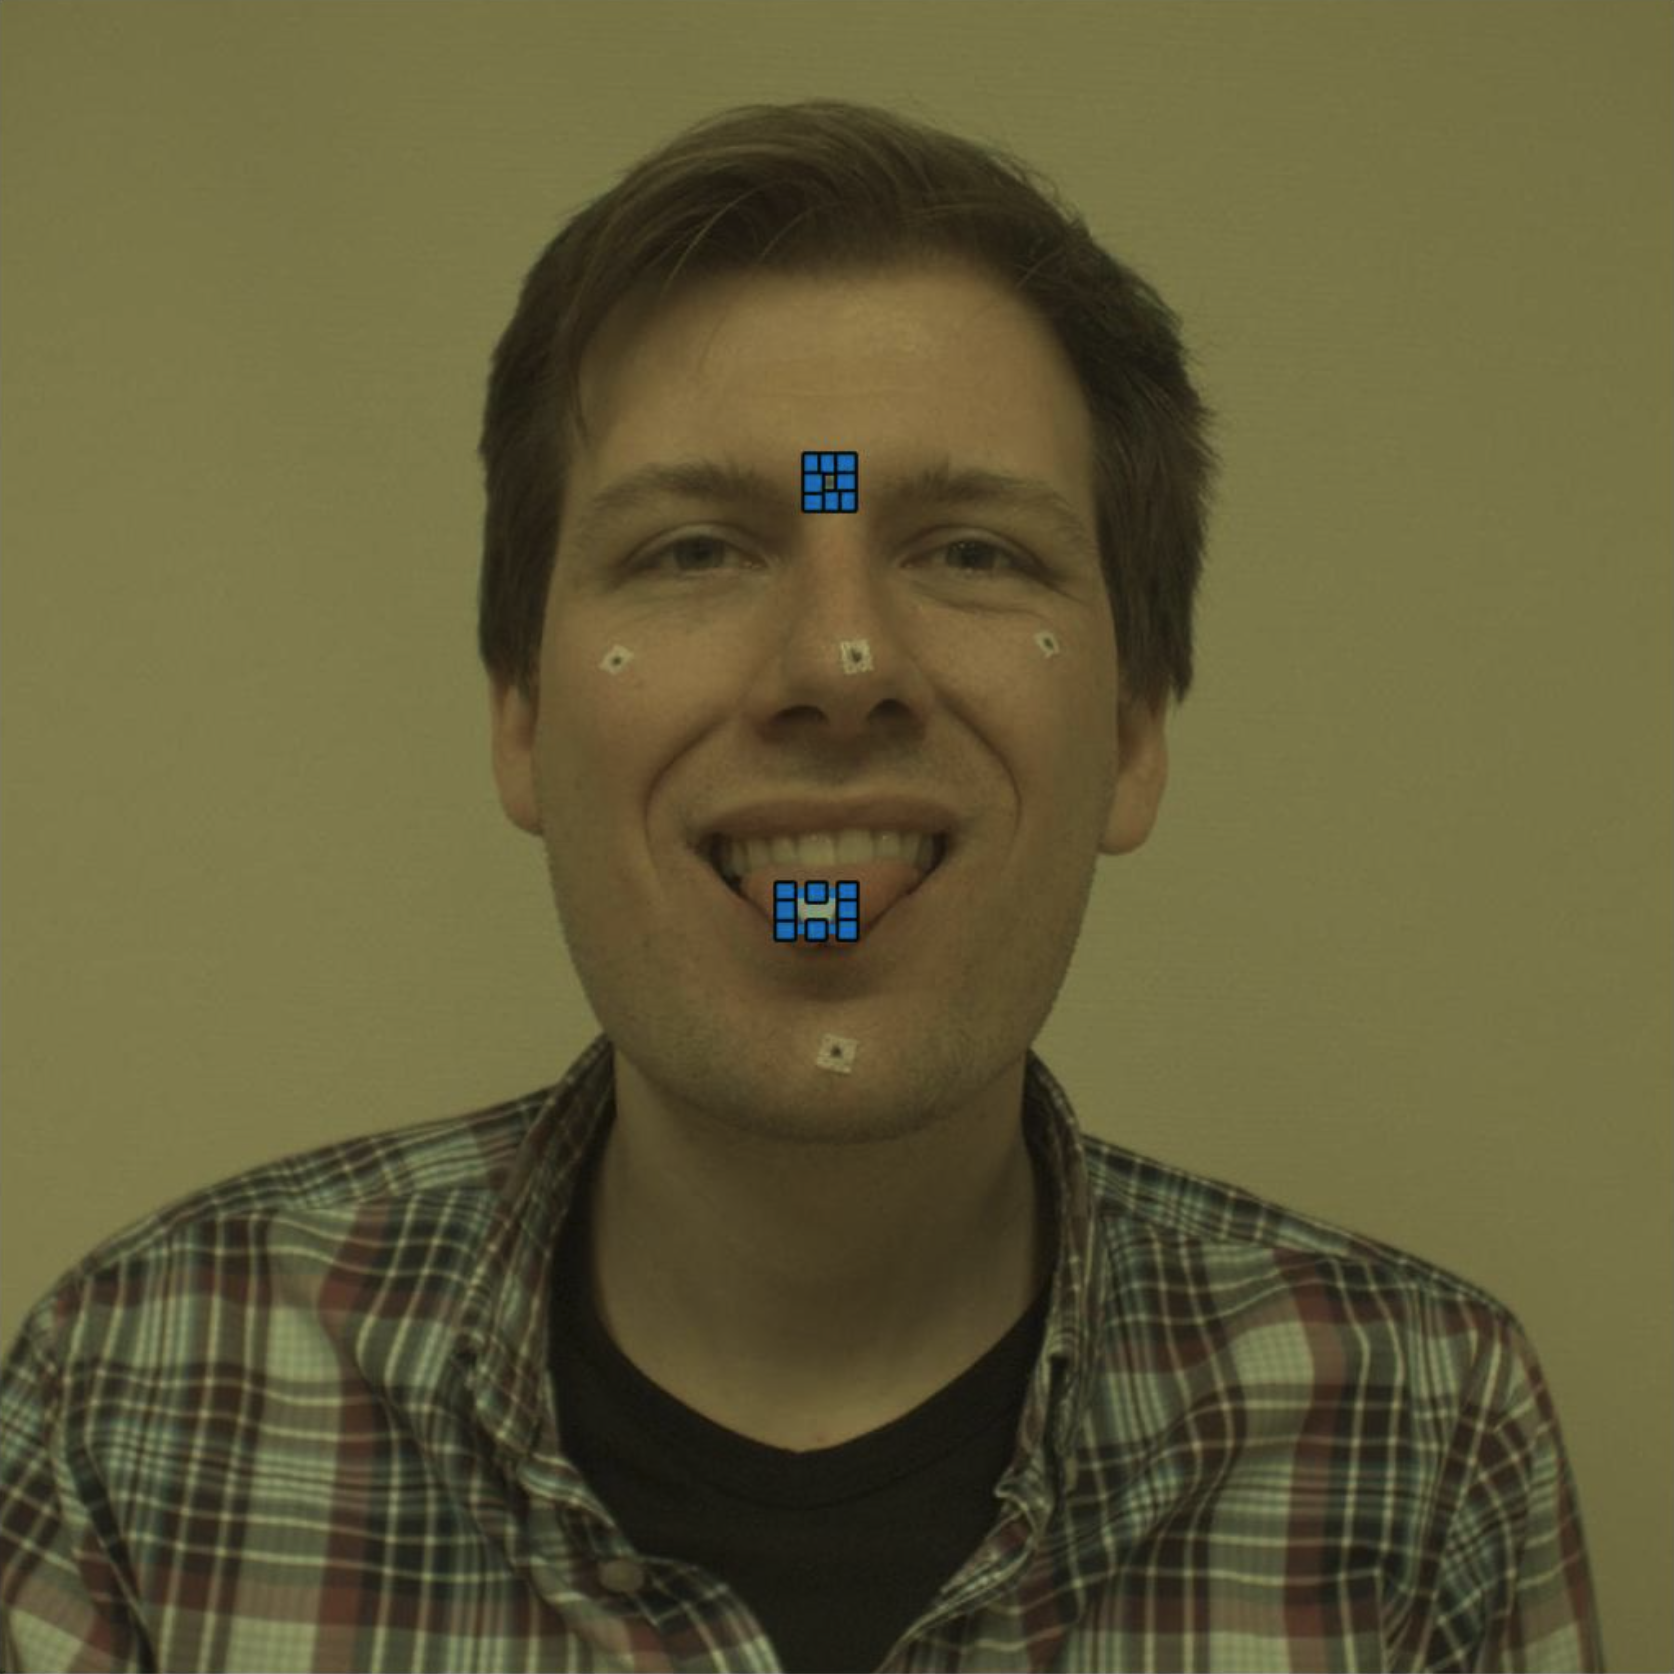
\includegraphics[width=1.5in]{figures/Select2ROI.png}%
\label{Two ROIs}}
\hfill
\subfloat[Three ROIs]{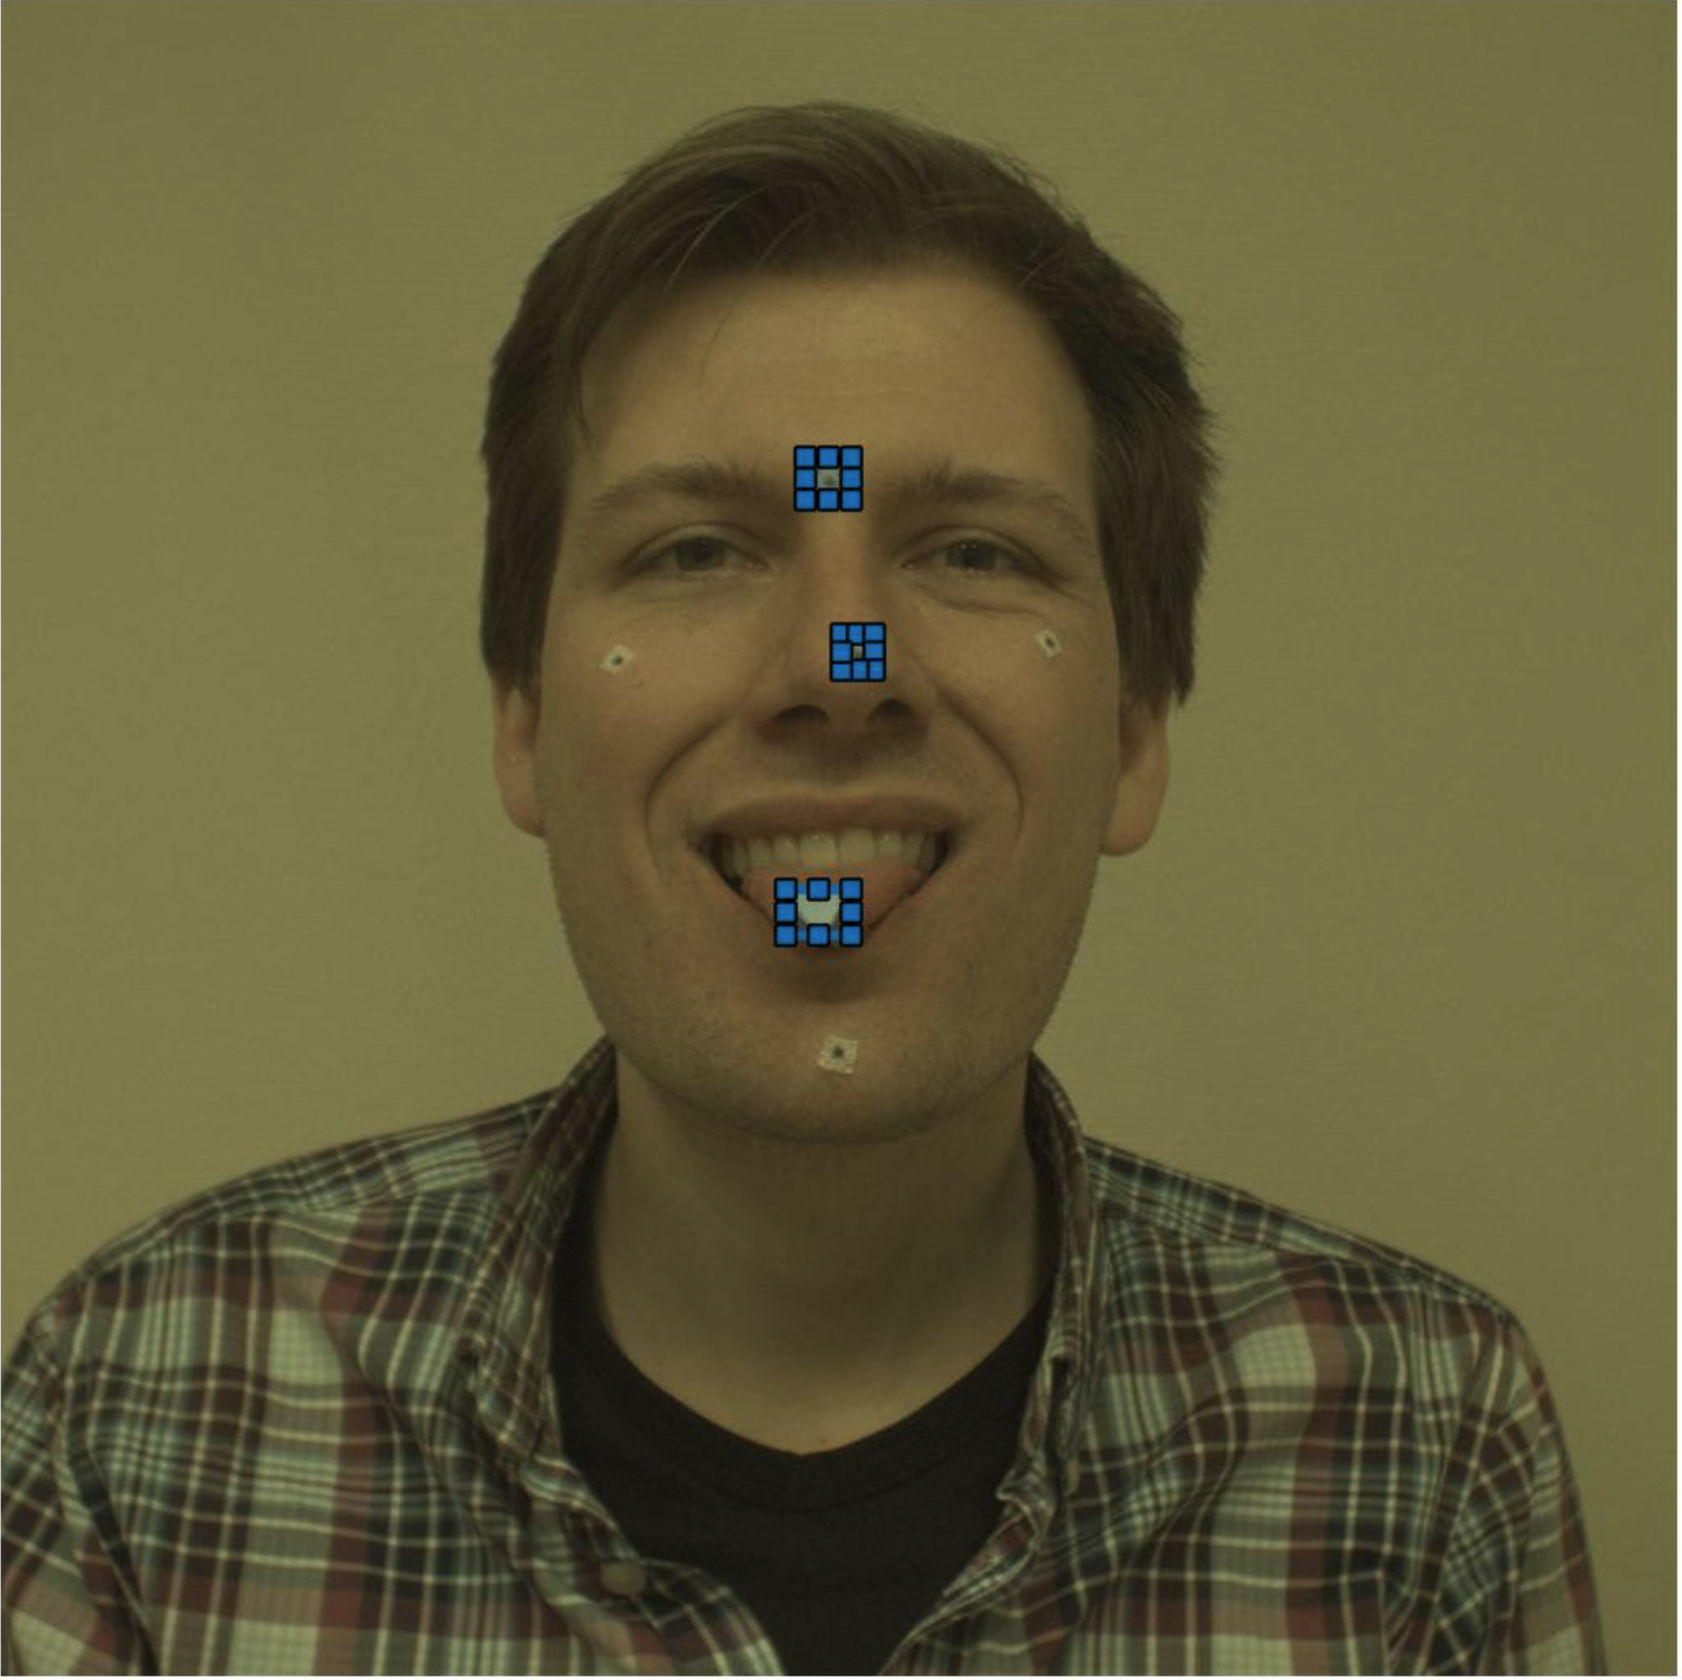
\includegraphics[width=1.5in]{figures/Select3ROI.png}%
\label{Three ROIs}} 
\\
\subfloat[Two ROIs with tracked points]{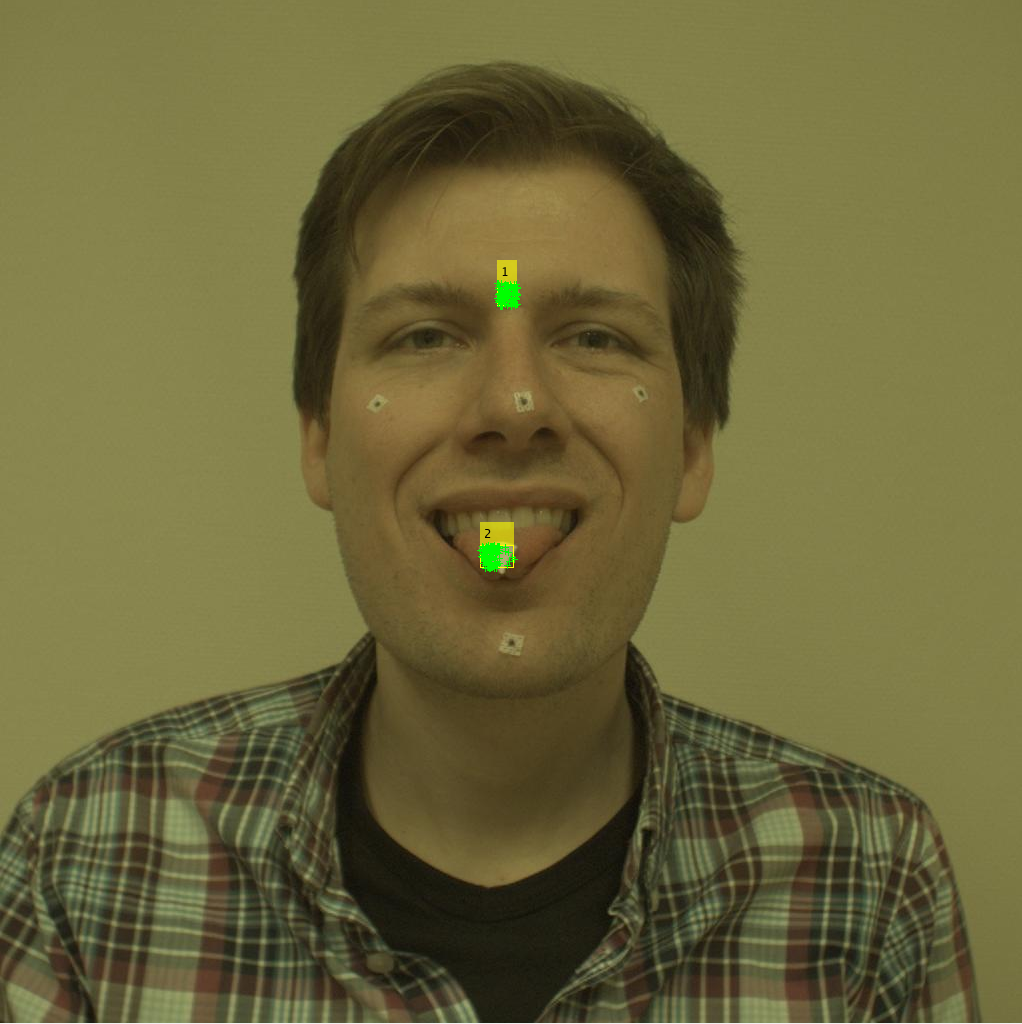
\includegraphics[width=1.5in]{figures/2ROIwithPoints.png}%
\label{2ROIwithPoints}}
\caption{Selected ROIs: two ROIs in (a) and three ROIs in (b). Two selected ROIs with the selected points inside them in (c)}
\label{select2ROI}
\end{figure}
 After selecting those ROIs, the minimum eigenvalue algorithm\footnote{This algorithm was chosen after simply comparing the number of points it can detect against other corner detectors that are available on Matlab like Harris–Stephens, BRISK and FAST algorithms.} is used to detect corners within the ROI and define them as interest points to track.
 
 However, the ROIs are relatively small and there is a very limited number of interest points that can be found using this algorithm. And because large displacements are expected at the tongue tip we will definitely lose many points along the way, random points inside the ROIs will be selected and also tracked to increase the overall number of the points that are tracked in each ROI as shown in Fig. \ref{2ROIwithPoints}. This set of points will be tracked using the Kanade-Lucas-Tomasi (KLT) tracking algorithm.
%  \begin{figure}[!t]
%  	\centering
%  	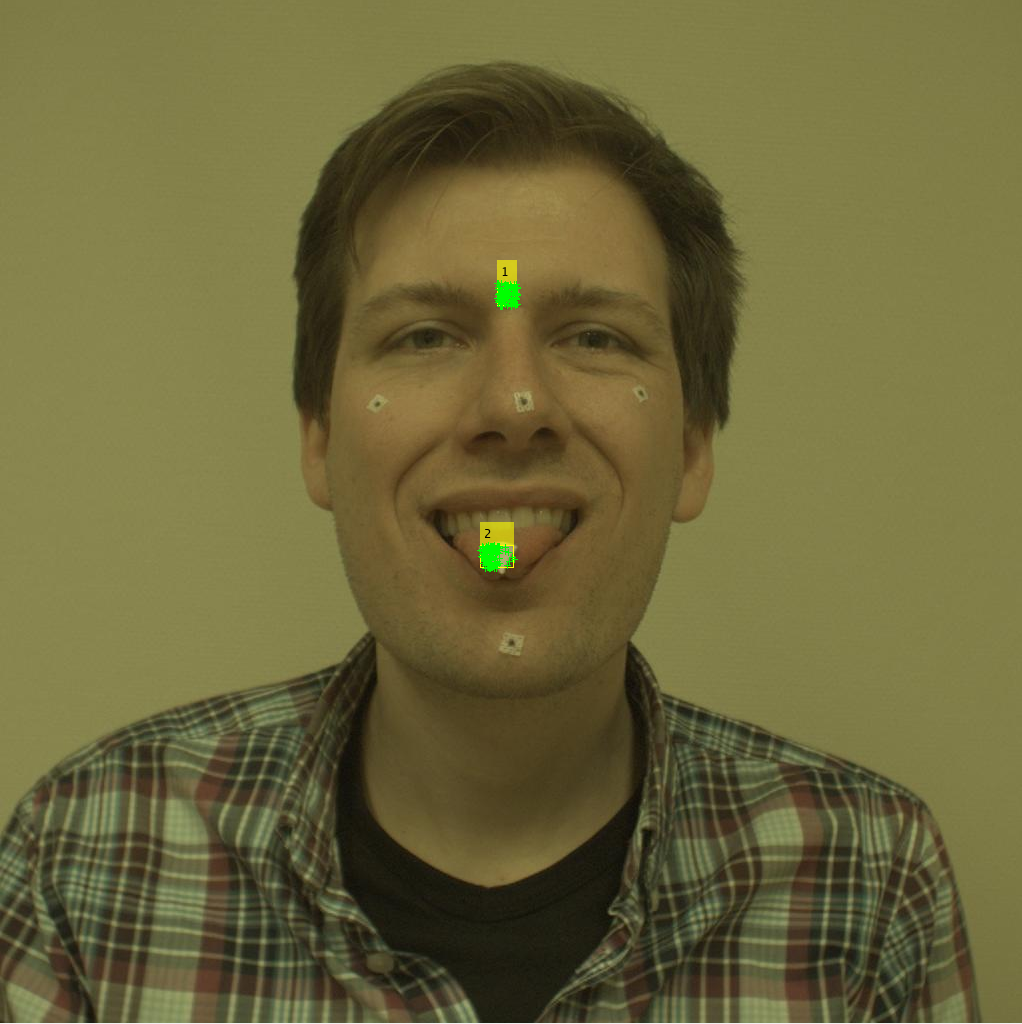
\includegraphics[width=0.2\textwidth]{figures/2ROIwithPoints.png}
%  	\caption{Two selected ROI with the selected points inside them}
%  	\label{2ROIwithPoints}
%  \end{figure}

\subsubsection{Kanade-Lucas-Tomasi Feature Tracker}
Kanade-Lucas-Tomasi Feature Tracker, to be referred to later as KLT tracker, is a tracking method based on \cite{KL} and \cite{KLT}. Where the algorithm tries to locate a set of points $P(x,y)$ in the image ($k+1$) given its 2D coordinates in the image ($k$). This method only tracks selected points from the set $P(x,y)$ and discards the other points as untrackable. The selection is based on eigenvalues of the gradient matrix at a given point, if the two eigenvalues are larger than some threshold the point will be tracked, otherwise, it will be discarded.

Therefore, it is almost guaranteed to lose all the tracked points if the tracking was done over a long series of images. So it is important to start with a large set of points $P(x,y)$ and reacquire points periodically. Also, if a large set of points is tracked and since there are large displacements at the tongue tip, some of the tracked points might be tracked incorrectly. Which makes it important to eliminate those outliers, and keep track of only the points that are within the ROI. This can be done using Random Sampling and Consensus (RANSAC).
\subsubsection{Random Sampling and Consensus}
RANSAC is a method of estimating parameters from an observed dataset. This dataset might contain outliers, the algorithm is capable of detecting those outliers and eliminate them so that they do not influence the estimation of the parameters. In the context of this project, RANSAC was used to detect and eliminate the outliers from the tracked dataset, and also to estimate the $(x,y)$ position of the ROIs, i.e. the reference point and tongue tip. After estimating the $(x,y)$ position of the ROIs at a given time and from two cameras in the pixel coordinates, we will be able to estimate the 3D position of these ROIs in the world coordinates using the camera parameters and triangulation.

\subsection{3D Tracking}
Estimating the $(x,y)$ positions of the ROIs in the pixel coordinates for a series of $n$ frames will provide us with the path of these ROIs along the series of $n$ frames. If we have this path (series of $(x,y)$ points for $n$ frames) for two cameras, we can estimate the 3D position of this series of points with respect to a world frame, this is done using triangulation and camera parameters that can be estimated using Camera Calibration methods.
\subsubsection{Camera Calibration}
To be able to transform a certain point $a_p(x,y)$ expressed in pixels coordinates to the world coordinates $a_W(x,y)$ you need to transform first from pixel coordinates to camera coordinates, then to world coordinates. The first transform is done using, what is called, intrinsics parameters, and the second is done using the extrinsics parameters.

These parameters can be estimated in a process called camera calibration. In camera calbiration, the calibrator is provided with a set of pictures of a checkerboard that has squares of known side length that is also is passed to the calibrator. The calibrator will then detect the corners of the checkerboard's squares and then estimate the parameter by solving the closed-form equation that relates the pixel coordinates to the world coordinates in a pinhole camera model:
\begin{equation} \label{CameraModel}
w\begin{bmatrix}
x & y & 1
\end{bmatrix} = 
\begin{bmatrix}
X & Y & Z & 1
\end{bmatrix}  
\begin{bmatrix}
R\\ t
\end{bmatrix} 
K
\end{equation}
Where:

$(X, Y, Z)$ are the world coordinates of the point.

$(x,y)$ are the pixel coordinates of the point.

$w$ is the homogeneous scale factor.

$K$ is the intrinsic parameters matrix.

$(R,t)$ are the rotation and translation of the camera with respect to the world coordinates, i.e. extrinsics parameters.

The calibrator can also estimate the lens distortion model, that can be used to undistort an image. After estimating the required parameters for the two cameras, we can estimate the $(X, Y, Z)$ of a certain ROIs in the world coordinates given a pair of matching points that represent the ROI in the two cameras. This is called Triangulation.
\subsubsection{Triangulation}
The two matched points $a(x_1 , y_1)$ and $b(x_2 , y_2)$, expressed in pixels coordinates of their respected cameras, together with the parameters for the two cameras can be used to estimate the $(X, Y, Z)$ of this point in the world coordinates. This is done using Linear triangulation from \cite{triangulation}. This step will provide us with a 3D reconstructed path of the ROIs. This 3D path will have the path of the fixed reference point and the path of the tongue tip, those two paths will be used to estimate the Range of Motion of the tongue tip.
\subsubsection{Range of Motion Estimation}
To be continued...
\section{Implementation}
In this section, the practical workflow of the system will be presented. The used platform is Matlab. The system is already redundant and has three cameras, left, right and middle camera. The two cameras that will be mainly used are Left and Middle cameras. The 2D paths generation is done by tracking the ROIs, estimating their $(x,y)$, and registering the coordinates. This will be done to the cameras, and then the 3D path can be reconstructed from the two 2D paths, to do that the camera parameters should be estimated first using Stereo Camera Calibrator App. Finally, the Range of Motion of the tongue tip can be estimated using the 3D path. 
\subsection{Multi-Object Tracking Class}
Based on \cite{matlabClass}, a Multi-Object Tracking Matlab Class \texttt{MultiObjectTrackerKLT} was developed to be used in this project. The class encapsulates a lot of the logistics of dealing with multiple ROIs. The class uses Matlab's KLT tracker \texttt{vision.PointTracker} and \texttt{{ut-ransac}}.
\subsection{2D Paths Generation}
%I Ayham will work on this. We select ROIs, we track them over many frames (eliminate outliers, repopulate), we have a path. We do this again to the second camera. we have two 2D paths.
First of all, the first frame is read, and the two ROIs will be selected as shown previously in Fig. \ref{select2ROI}. When those two ROIs are selected, the system will detect the corner points using the \texttt{detectMinEigenFeatures} and then generate a number of random points to track inside each ROI, as shown i Fig. \ref{2ROIwithPoints}. All of these points will be registered to be tracked in the next frame.
\begin{figure}[!t]
	\centering
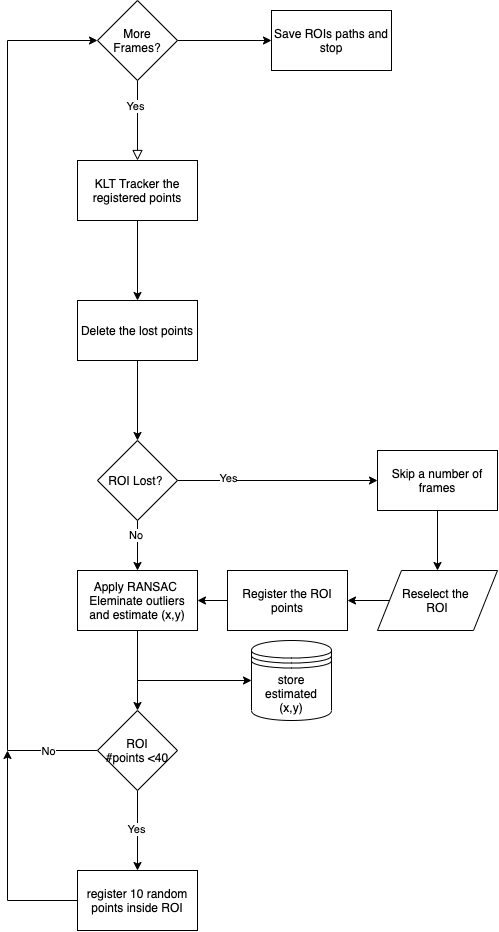
\includegraphics[width=0.85\linewidth]{Report/figures/Tracker_FChart.png}
\caption{Flow chart of the tracking algorithm}
\label{iteration_FChart}
\end{figure}
After that, the system will iterate until the video have no more frames, as shown in Fig. \ref{iteration_FChart}. The next frame is read, the tracker tries to locate the registered points, the lost points are deleted. If all the points from an ROI are lost as in Fig. \ref{ROILost}, the system will skip some frames, and then stop until the user selects the ROI again, as in Fig. \ref{Reselect}. RANSAC is applied to the remaining points of each ROI to eliminate the outliers, as shown in Fig. \ref{RANSAC} and estimate the $(x,y)$ of each ROI, if the remaining inliers inside an ROI are less than a certain number (40), a number of random points (10) which are inside the ROI will be registered to be tracked next iteration as shown in Fig. \ref{repopulate}.
After applying this to the videos from the middle and left camera, 2D Paths of the two ROIs will be obtained as shown in Fig. \ref{2PathsML}.

\begin{figure}[!t]
	\centering
\subfloat[]{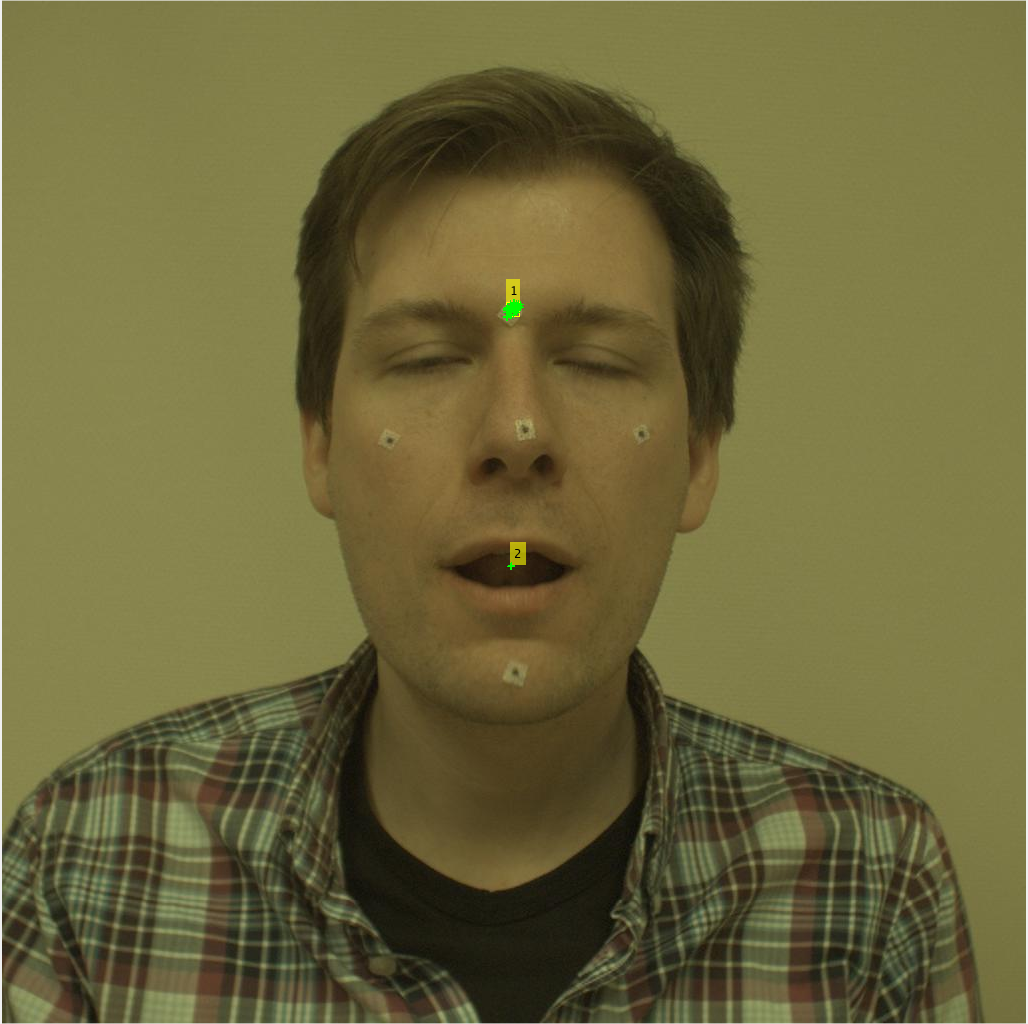
\includegraphics[width=0.45\linewidth]{Report/figures/ROILost.png}%
\label{ROILost}}
\hfill
\subfloat[]{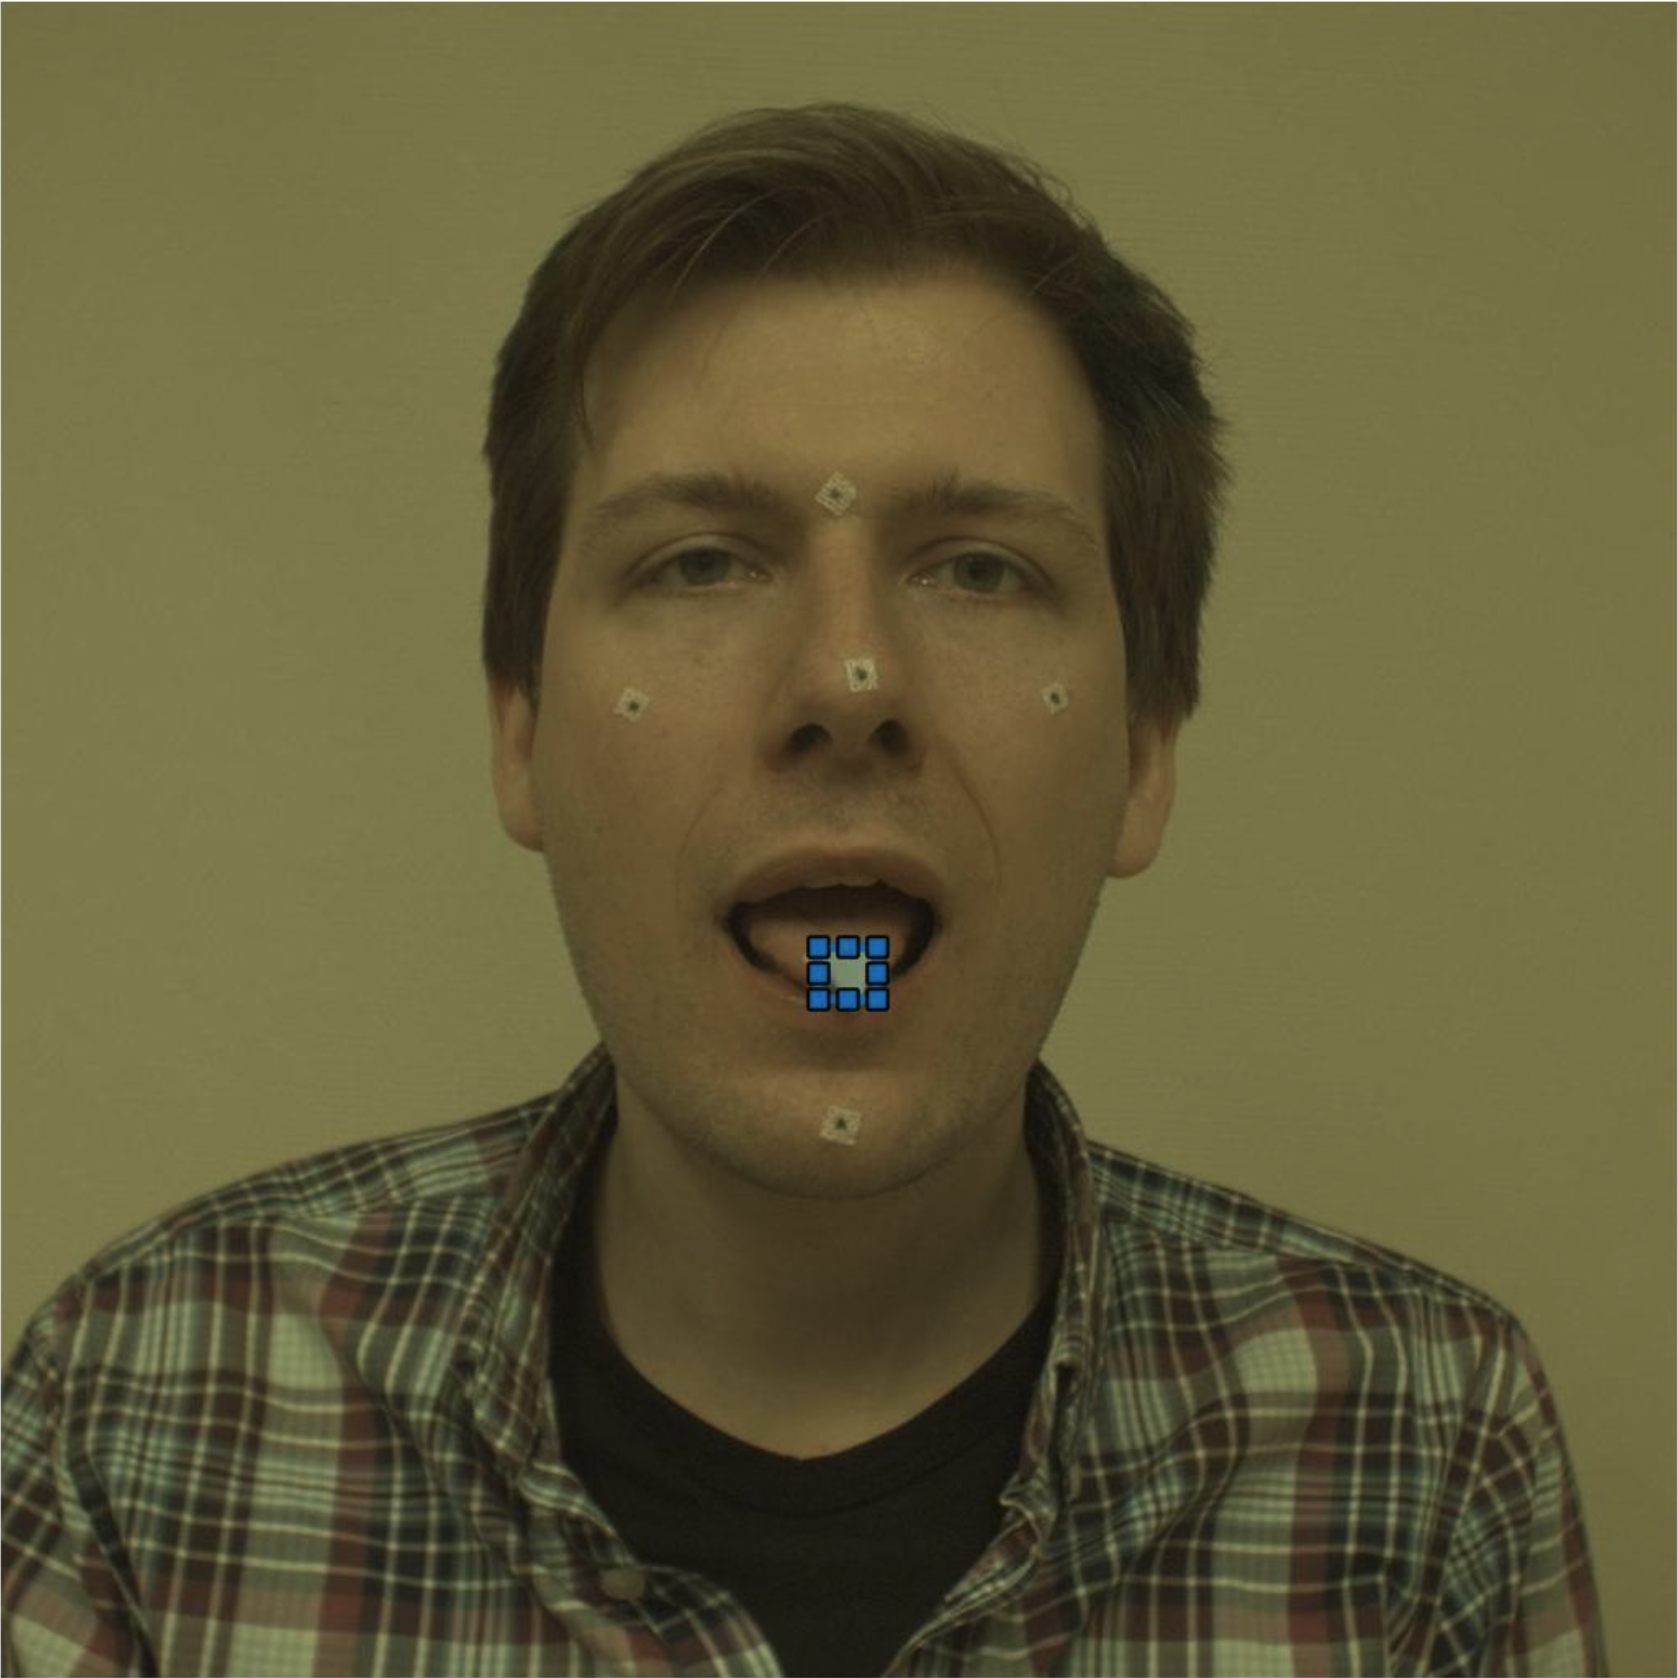
\includegraphics[width=0.45\linewidth]{Report/figures/ReselectROI.png}%
\label{Reselect}} 
\caption{(a) one ROI is lost. (b) The lost ROI is re-selected}
\label{ReSelectROI}
\end{figure}
\begin{figure}[!t]
	\centering
\subfloat[]{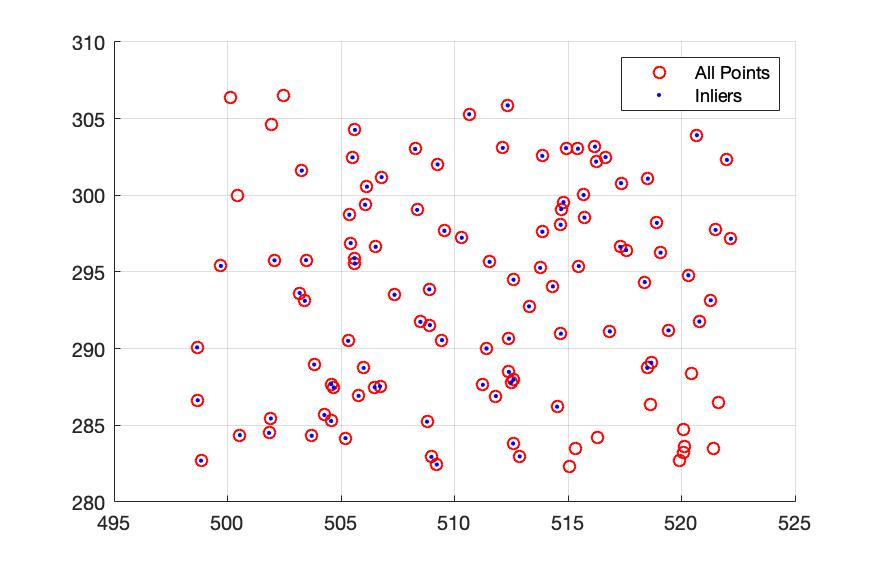
\includegraphics[width=0.49\linewidth]{Report/figures/RANSAC.jpg}%
\label{RANSAC}}
\hfill
\subfloat[]{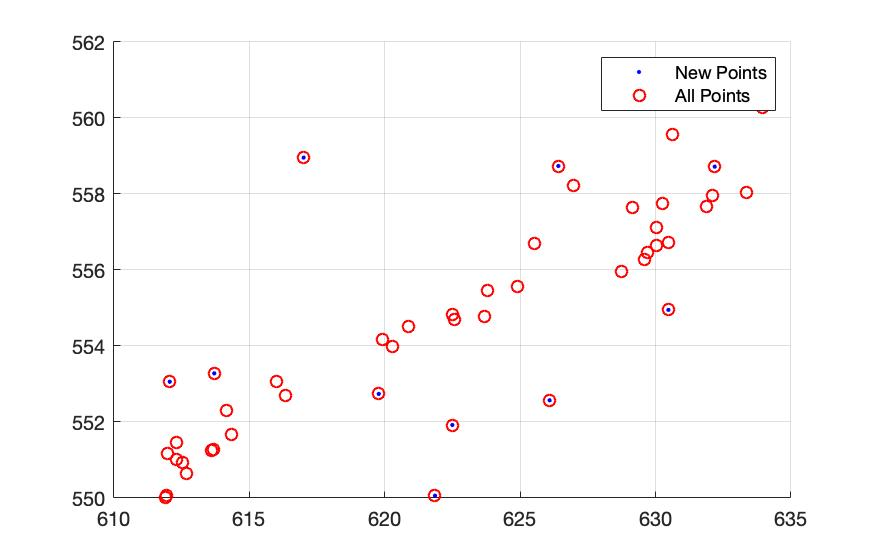
\includegraphics[width=0.49\linewidth]{Report/figures/repopulate.jpg}%
\label{repopulate}} 
\caption{(a) RANSAC applied to a dataset. (b) Random points are added to the small dataset}
\label{methodsRANSAC_repopulate}
\end{figure}
\begin{figure}[!t]
	\centering
\subfloat[]{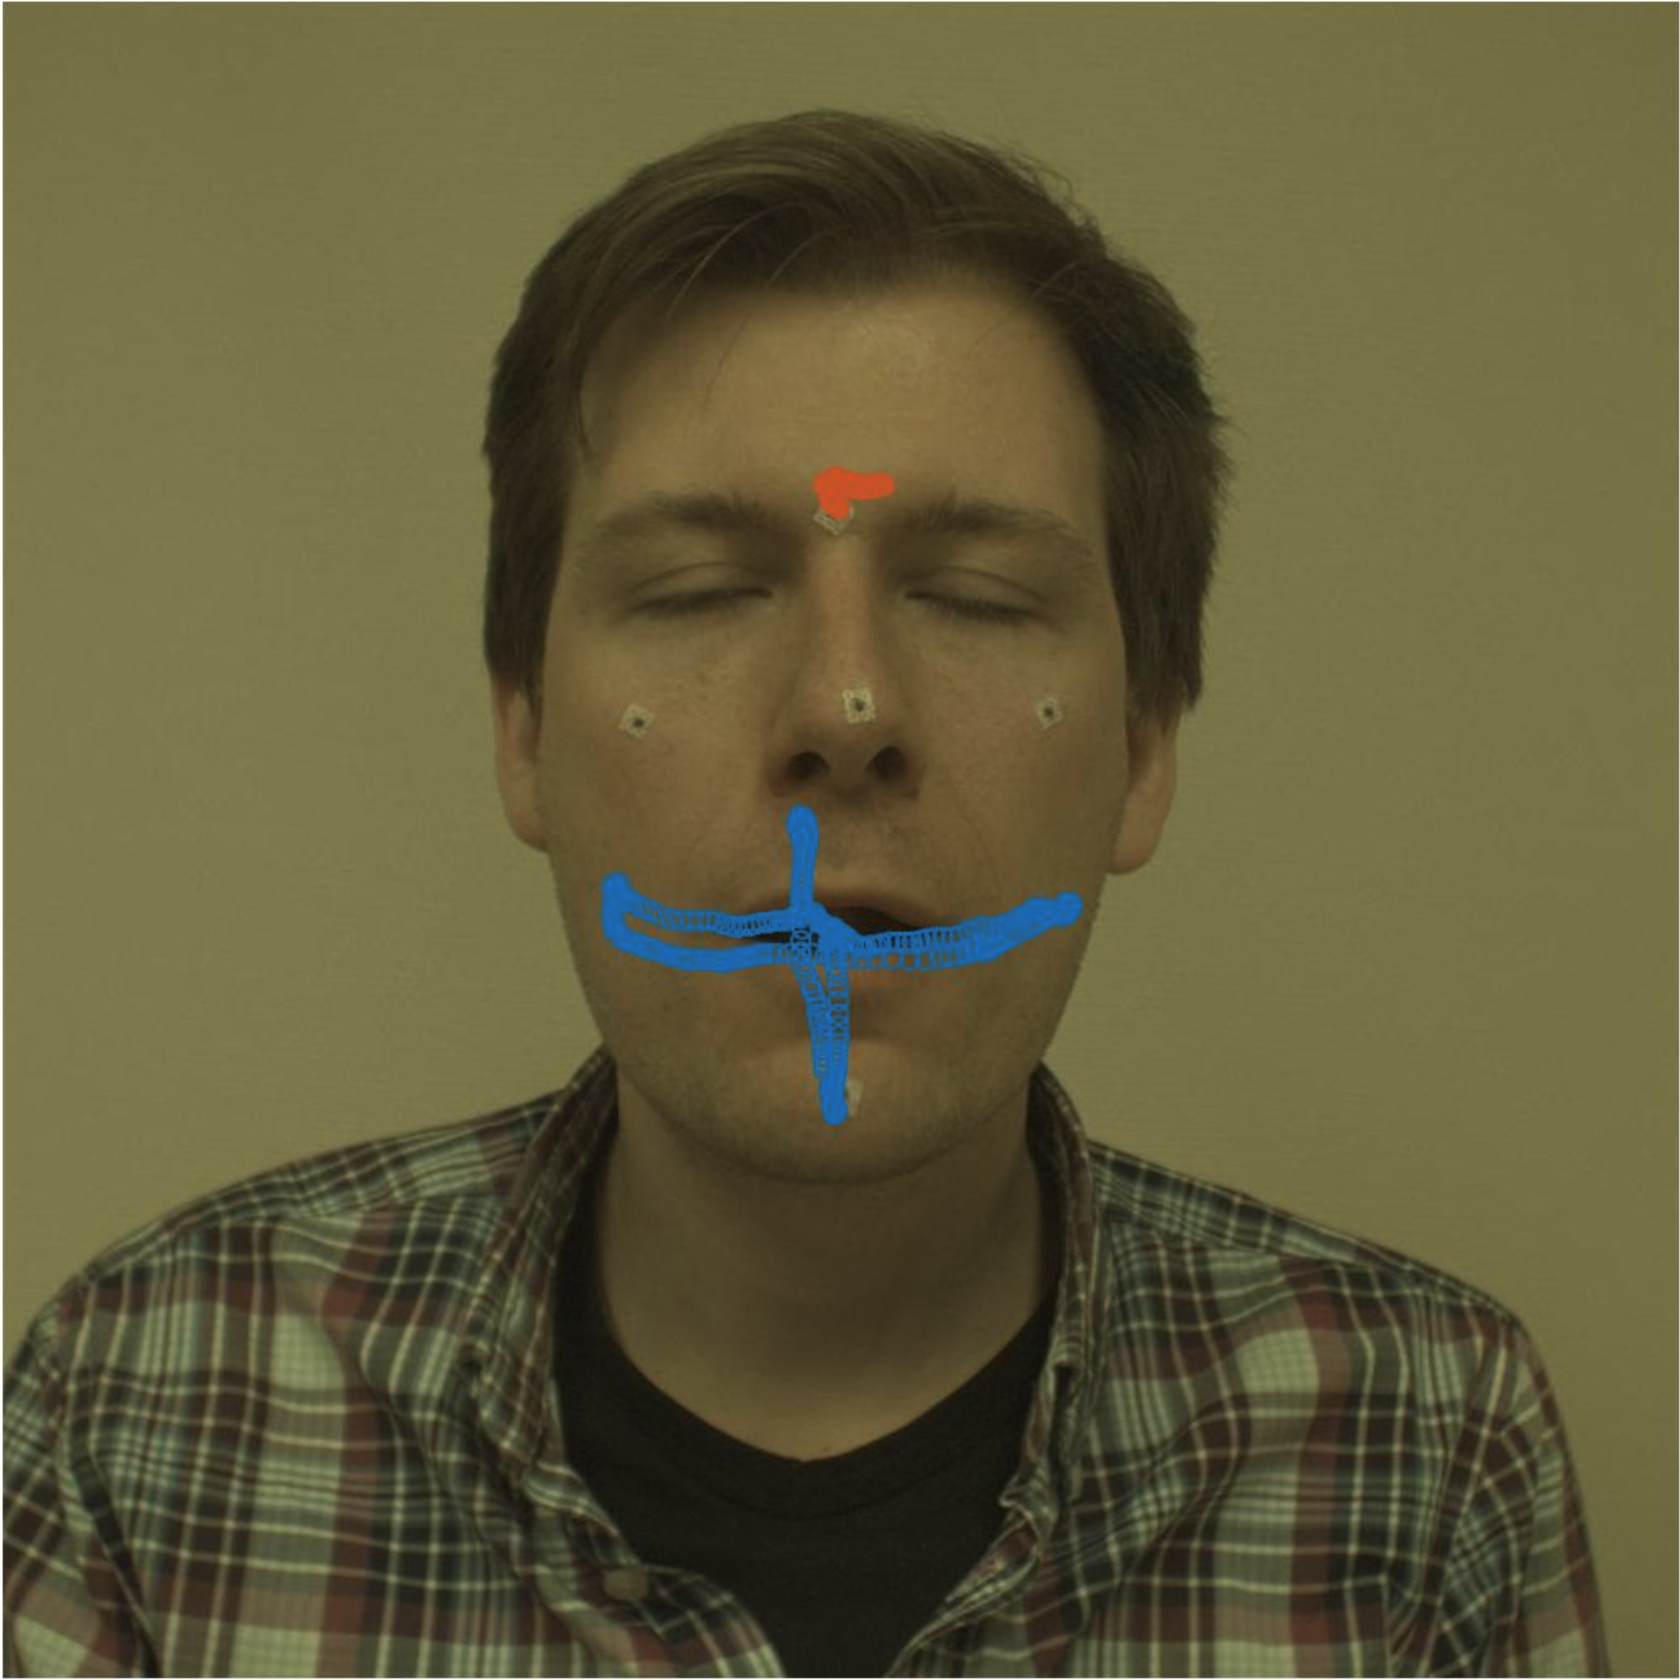
\includegraphics[width=0.45\linewidth]{Report/figures/framewithPathsM.png}%
\label{2PathM}}
\hfill
\subfloat[]{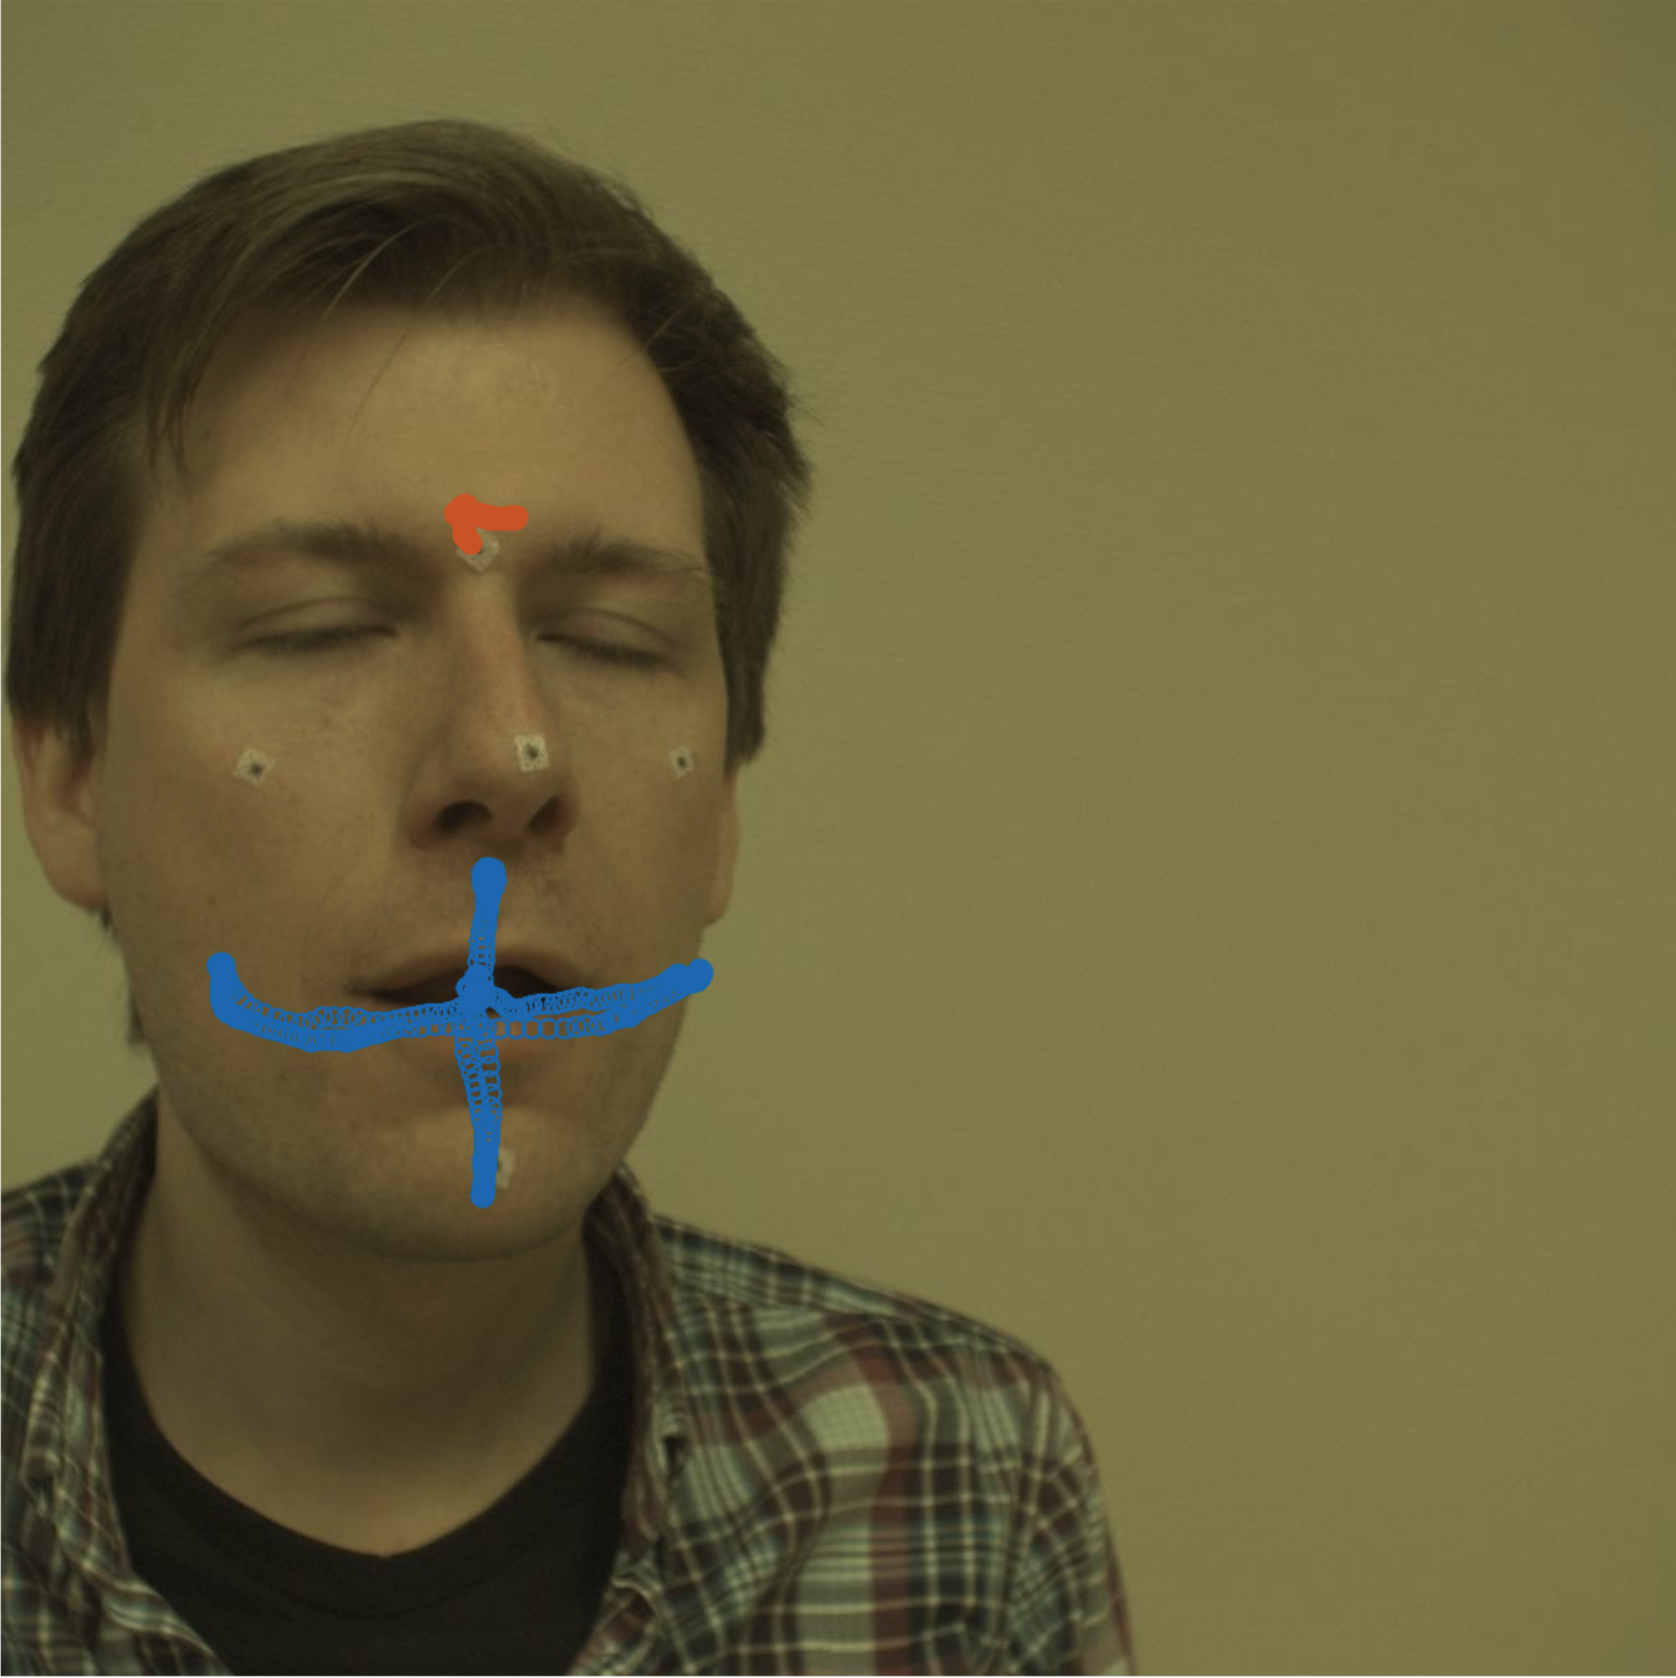
\includegraphics[width=0.45\linewidth]{Report/figures/framewithPathsL.png}%
\label{2PathL}} 
\caption{2D paths of two ROI from (a) Middle camera. (b) Left camera.}
\label{2PathsML}
\end{figure}

\subsection{3D Path Reconstruction}
%We estimate camera parameter (figures Matlab's \texttt{stereoCameraCalibrator}), then we triangulate the paths, then 3D Path (Figures).

The tracking points will generate a path over time, where each time step is the reciprocal of the frame rate. Given that the input videos are 100 FPS, the $\Delta t = \frac{1}{100} s = 10 ms$. This appears to be enough resolution to create an acceptable path in each of the camera's views, yielding three 2D paths - and thus three pairs of 2D paths -  that can be used to reconstruct a 3D path, with two other 3D paths for redundancy. As the leftmost camera and rightmost camera have the biggest difference in angle relative to one another, the depth estimation should be most precise using this 2D path pair. However, since it also introduces more occlusion, for example by the nose, points of the other pairs could be used to fill in these gaps. We have not done so in this case, but is feasible.

In order to reconstruct the 3D path, the parameters or each camera has to be known. For this, we used the \texttt{stereoCameraCalibrator} along with the provided checkerboard images to initialise all three possible camera pairs, as shown in Fig. \ref{stereo}. Then, with two 2D paths and the respective \texttt{stereoParameters} file, it is possible to visualise the tongue tracker's path. The same can be done for the facial markers. To achieve this smoothly, the function \texttt{create3DPath} was created. It takes in two $N\times2$ arrays of $(x,y)$ pairs, and the accompanying \texttt{stereoParams} file. The function, in turn, uses the \texttt{triangulate} function, which is a function of Matlab's Computer Vision System Toolbox. It returns an array of $N\times3$ that have the 3D coordinates $(x,y,z)$ of the points, which is its horizontal and vertical distance, and its depth away from the center of the first camera of which the path was put into \texttt{triangulate}. 

The construction needs to be repeated for the tracker at the top of the bridge of the user's nose, which will be used as the origin point of the coordinate frame. Subtracting the 3D path of the new origin point from the path of the tongue will give us this system.

\begin{figure}[!t]
	\centering
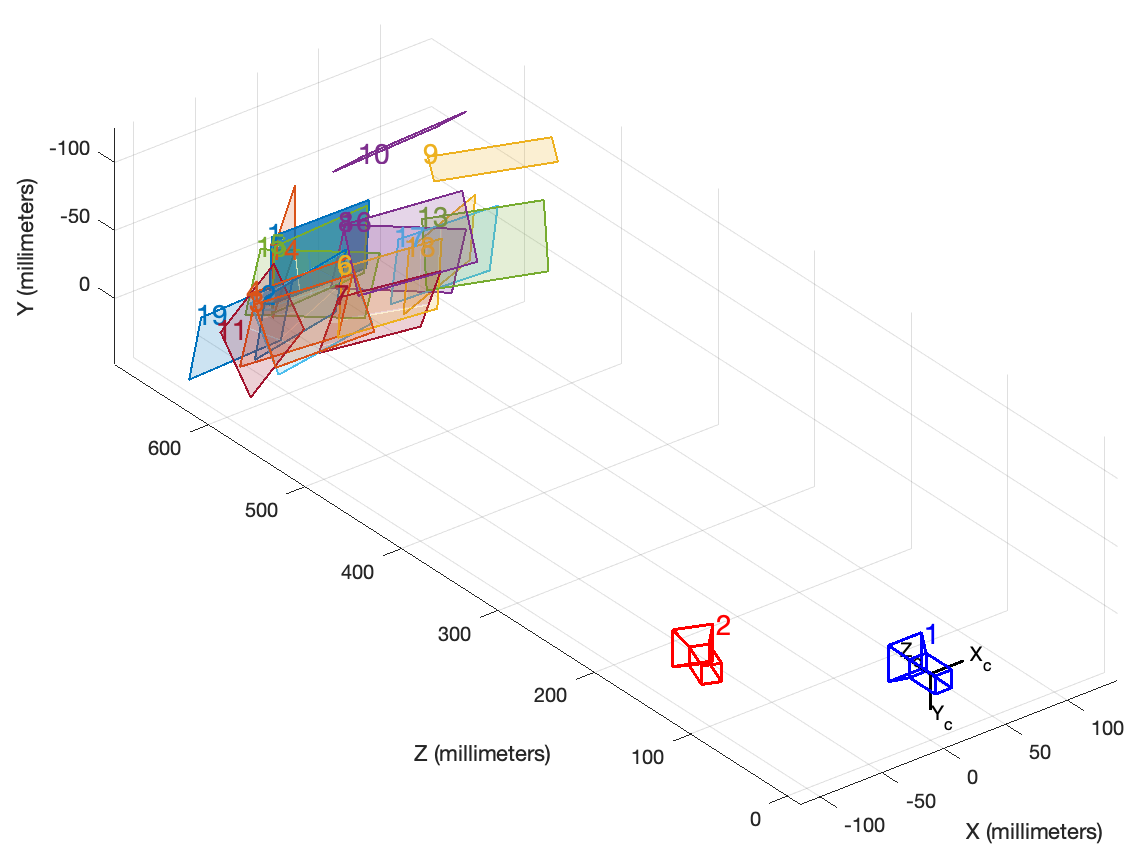
\includegraphics[width=0.75\linewidth]{Report/figures/StereoML.png}
\caption{Stereo Camera calibration of middle and left cameras}
\label{stereo}
\end{figure}
\begin{figure}[!t]
	\centering
\subfloat[]{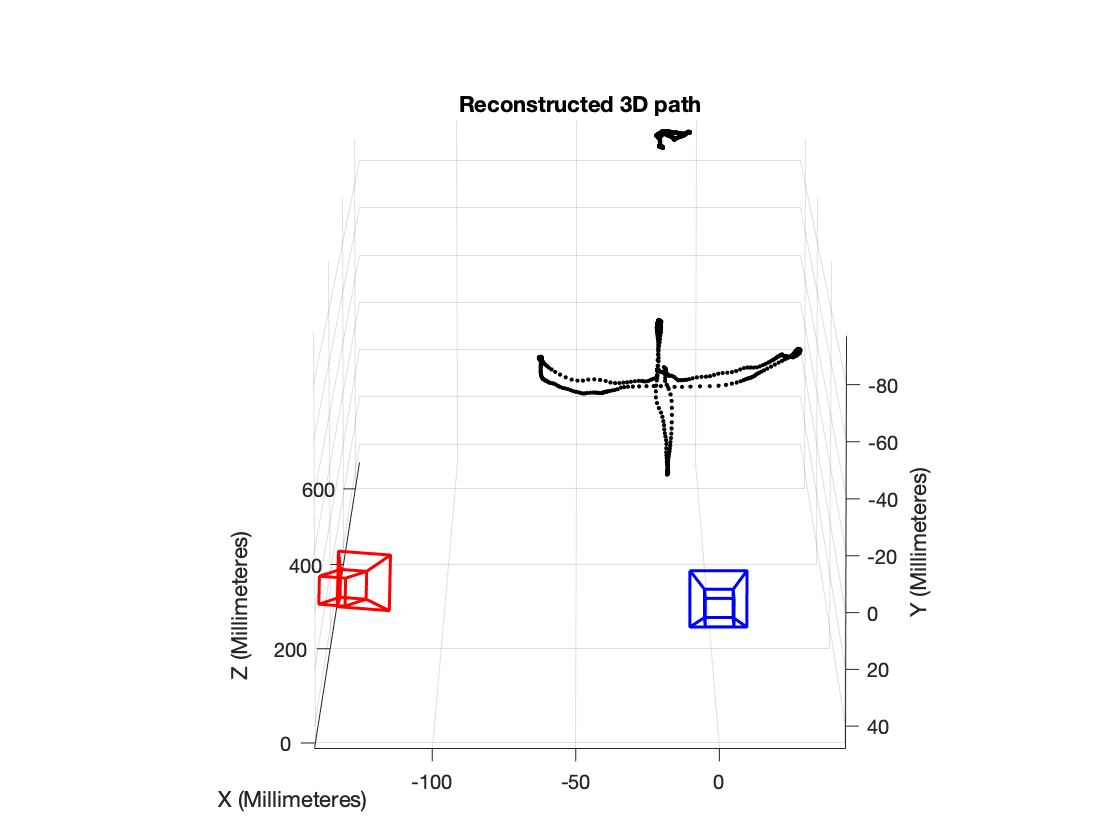
\includegraphics[width=0.8\linewidth]{Report/figures/3dML.png}%
\label{3DPathML}}
\hfill
\subfloat[]{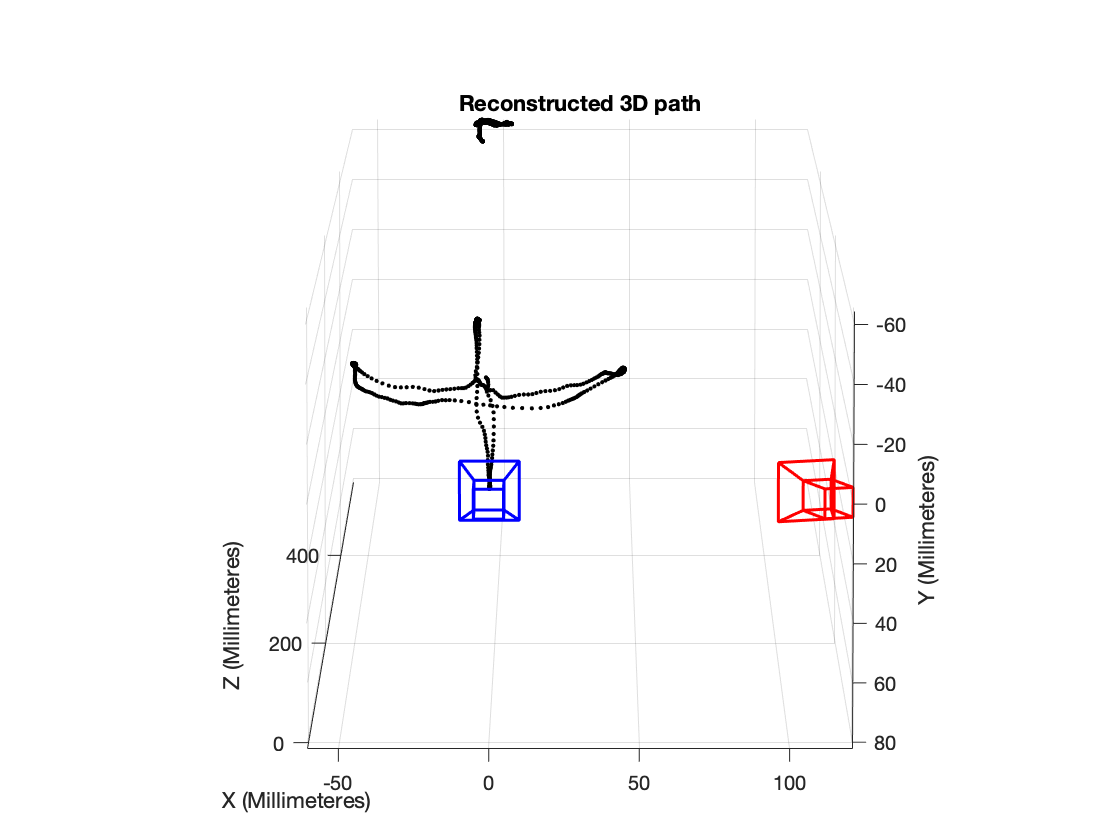
\includegraphics[width=0.8\linewidth]{Report/figures/3dMR.png}%
\label{3DPathMR}} 
\caption{3D reconstructed paths from (a) Middle and left cameras. (b) Middle and right cameras. Where the middle camera is the primary camera and the origin of 3D space}
\label{3Paths}
\end{figure}


\subsection{Range of Motion Estimation}
Finally, in order to estimate the Range of Motion, the motion should be decomposed into the basis vectors of the coordinate systems that form the x-axis, y-axis and z-axis. The x-axis is perfectly horizontal and the z-axis is straight up, assuming the cameras used to record the 2D paths are perfectly level in the x-axis and straight up on the z-axis on its tripod base or ball bearing. Note that this will yield the basis vectors for the camera that shot the video which forms the first argument in the \texttt{triangulation()} function. That is, if the path as seen from the left camera is the first argument in \texttt{triangulation()}, then the 3D path will be visualised as seen from the optical center of the left camera, and the basis vector will also be relative to the left camera. In short, this assumes that the basis vectors \emph{i}, \emph{j}, and \emph{k} are $<1, 0, 0>$, $<0, 1, 0>$, and $<0, 0, 1>$, respectively.

Horizontal movement of the tongue can be expressed a signed floating point number. If the sign is negative, the tip of the tongue is on the left side of the nose, as seen from the camera. If the sign if positive, the tip of the tongue is on the right side. The magnitude or absolute value of this number indicates its horizontal distance away from the nose.
Vertical movement of the tongue can be expressed as an unsigned floating point number. As the tongue is not able to travel above the top of the bridge of the nose, this number will always be positive in our reference frame. Again, the magnitude or absolute value will determine its vertical distance away from the reference point.
Movement in the z-direction will be a signed floating point number as well, and have similar characteristic as the horizontal movement.

Then, the points along the path can be decomposed as follows:

$x = (X, Y, Z)  \cdot <1, 0, 0>$

$y = (X, Y, Z)  \cdot <0, 1, 0>$

$z = (X, Y, Z)  \cdot <0, 0, 1>$

\section{Results}
We did this and that and here are the final results, figure of 2d paths form two camera, 3d path figure, range of motion plot.

While the system have acceptable results when the subject in the video is wearing paper tracker on the tongue tip and interest points on the face, many experiments have been done to test the system on the a subject without the paper trackers and the system failed to deliver a consistent and acceptable performance.
\section{Discussion}
Talk about the performance with tracker. Good, Acceptable, maybe better to track two cameras simultaneously, maybe better pre-processing? more effort on detecting the angles on the tongue tip?

The performance of the system can be improved by implementing an Optical Flow Estimator of the area around the mouth. Since the tongue tip have by far the largest displacements from any of its surroundings, it can be used to correct/verify the KLT tracker, this would be very beneficial especially for subjects without paper trackers. Unfortunately, we did not had time to test that. Also, 
\section{Conclusion}
A conclusion reviews the main points of the paper. Describe the overall implication of the results to the original problem statement (or research questions). Do not replicate the abstract as the conclusion. A conclusion might also elaborate on the importance of the work, or suggest applications.
% \appendices
% \section{Guidelines for formatting Math}
% If you are using Word, use either the Microsoft Equation Editor or the MathType add-on (\href{http://www.mathtype.com\#http://www.mathtype.com}{http://www.mathtype.com}) for equations in your paper. 

% Number equations consecutively with equation numbers in parentheses flush with the right margin, as in (\ref{eq:fourier}). Punctuate equations when they are part of a sentence, as in

% \begin{equation} \label{eq:fourier}
% f_n=\sum_{m=0}^{N-1}{F_mexp(2\pi \mathbf{j}\frac{ nm}{N}).}
% \end{equation}

% Be sure that the symbols in your equation have been defined before the equation appears or immediately following. Italicize symbols ($T$ might refer to temperature, but T is the unit tesla). Refer to (1), not eq. (1) or equation (1),  except at the beginning of a sentence: Equation (1) is ... . 


% \section{Guidelines for Graphs and Tables}
% \subsection{Graphs and Images}
% Below each figure (graph or image) there must be a caption with a figure number and a figure title. See Fig 1. Figure titles should be legible, approximately 8 to 10 point type. Each figure should be referenced in the text. Each axis of a graph should have a label. Use words rather than symbols. As an example, write the quantity Wavelength,  or Wavelength $\lambda$,  not just $\lambda$.  Put units in parentheses. Do not label axes only with units. As in Fig. \ref{fig:example}, for example, write Wavelength (nm),  not just (nm).  

% \subsection{Tables} 
% Tables should have a table caption on top. See Table \ref{tab:example}. Tables should be numbered with Roman Numerals (I, II, III, IV, and so on). Tables should also always be referenced in the text.

% \subsection{Videos}
% Videos should be uploaded as separate files. The preferred video format is mp4. Dont make the video files unnecessarily large. 20 Mbytes is acceptable, but 200 Mbyte is not. Appendix A contains a Matlab script that you can use to resize the frame size of a video. The parameter $quality$ controls the amount of compression. Sometimes it is also useful to skip frames. For instance, only write the odd frames to the output video. 

% An example of a floating figure using the graphicx package.
% Note that \label must occur AFTER (or within) \caption.
% For figures, \caption should occur after the \includegraphics.
% Note that IEEEtran v1.7 and later has special internal code that
% is designed to preserve the operation of \label within \caption
% even when the captionsoff option is in effect. However, because
% of issues like this, it may be the safest practice to put all your
% \label just after \caption rather than within \caption{}.
%
% Reminder: the "draftcls" or "draftclsnofoot", not "draft", class
% option should be used if it is desired that the figures are to be
% displayed while in draft mode.
%
% \begin{figure}[!t]
%         \centering
%         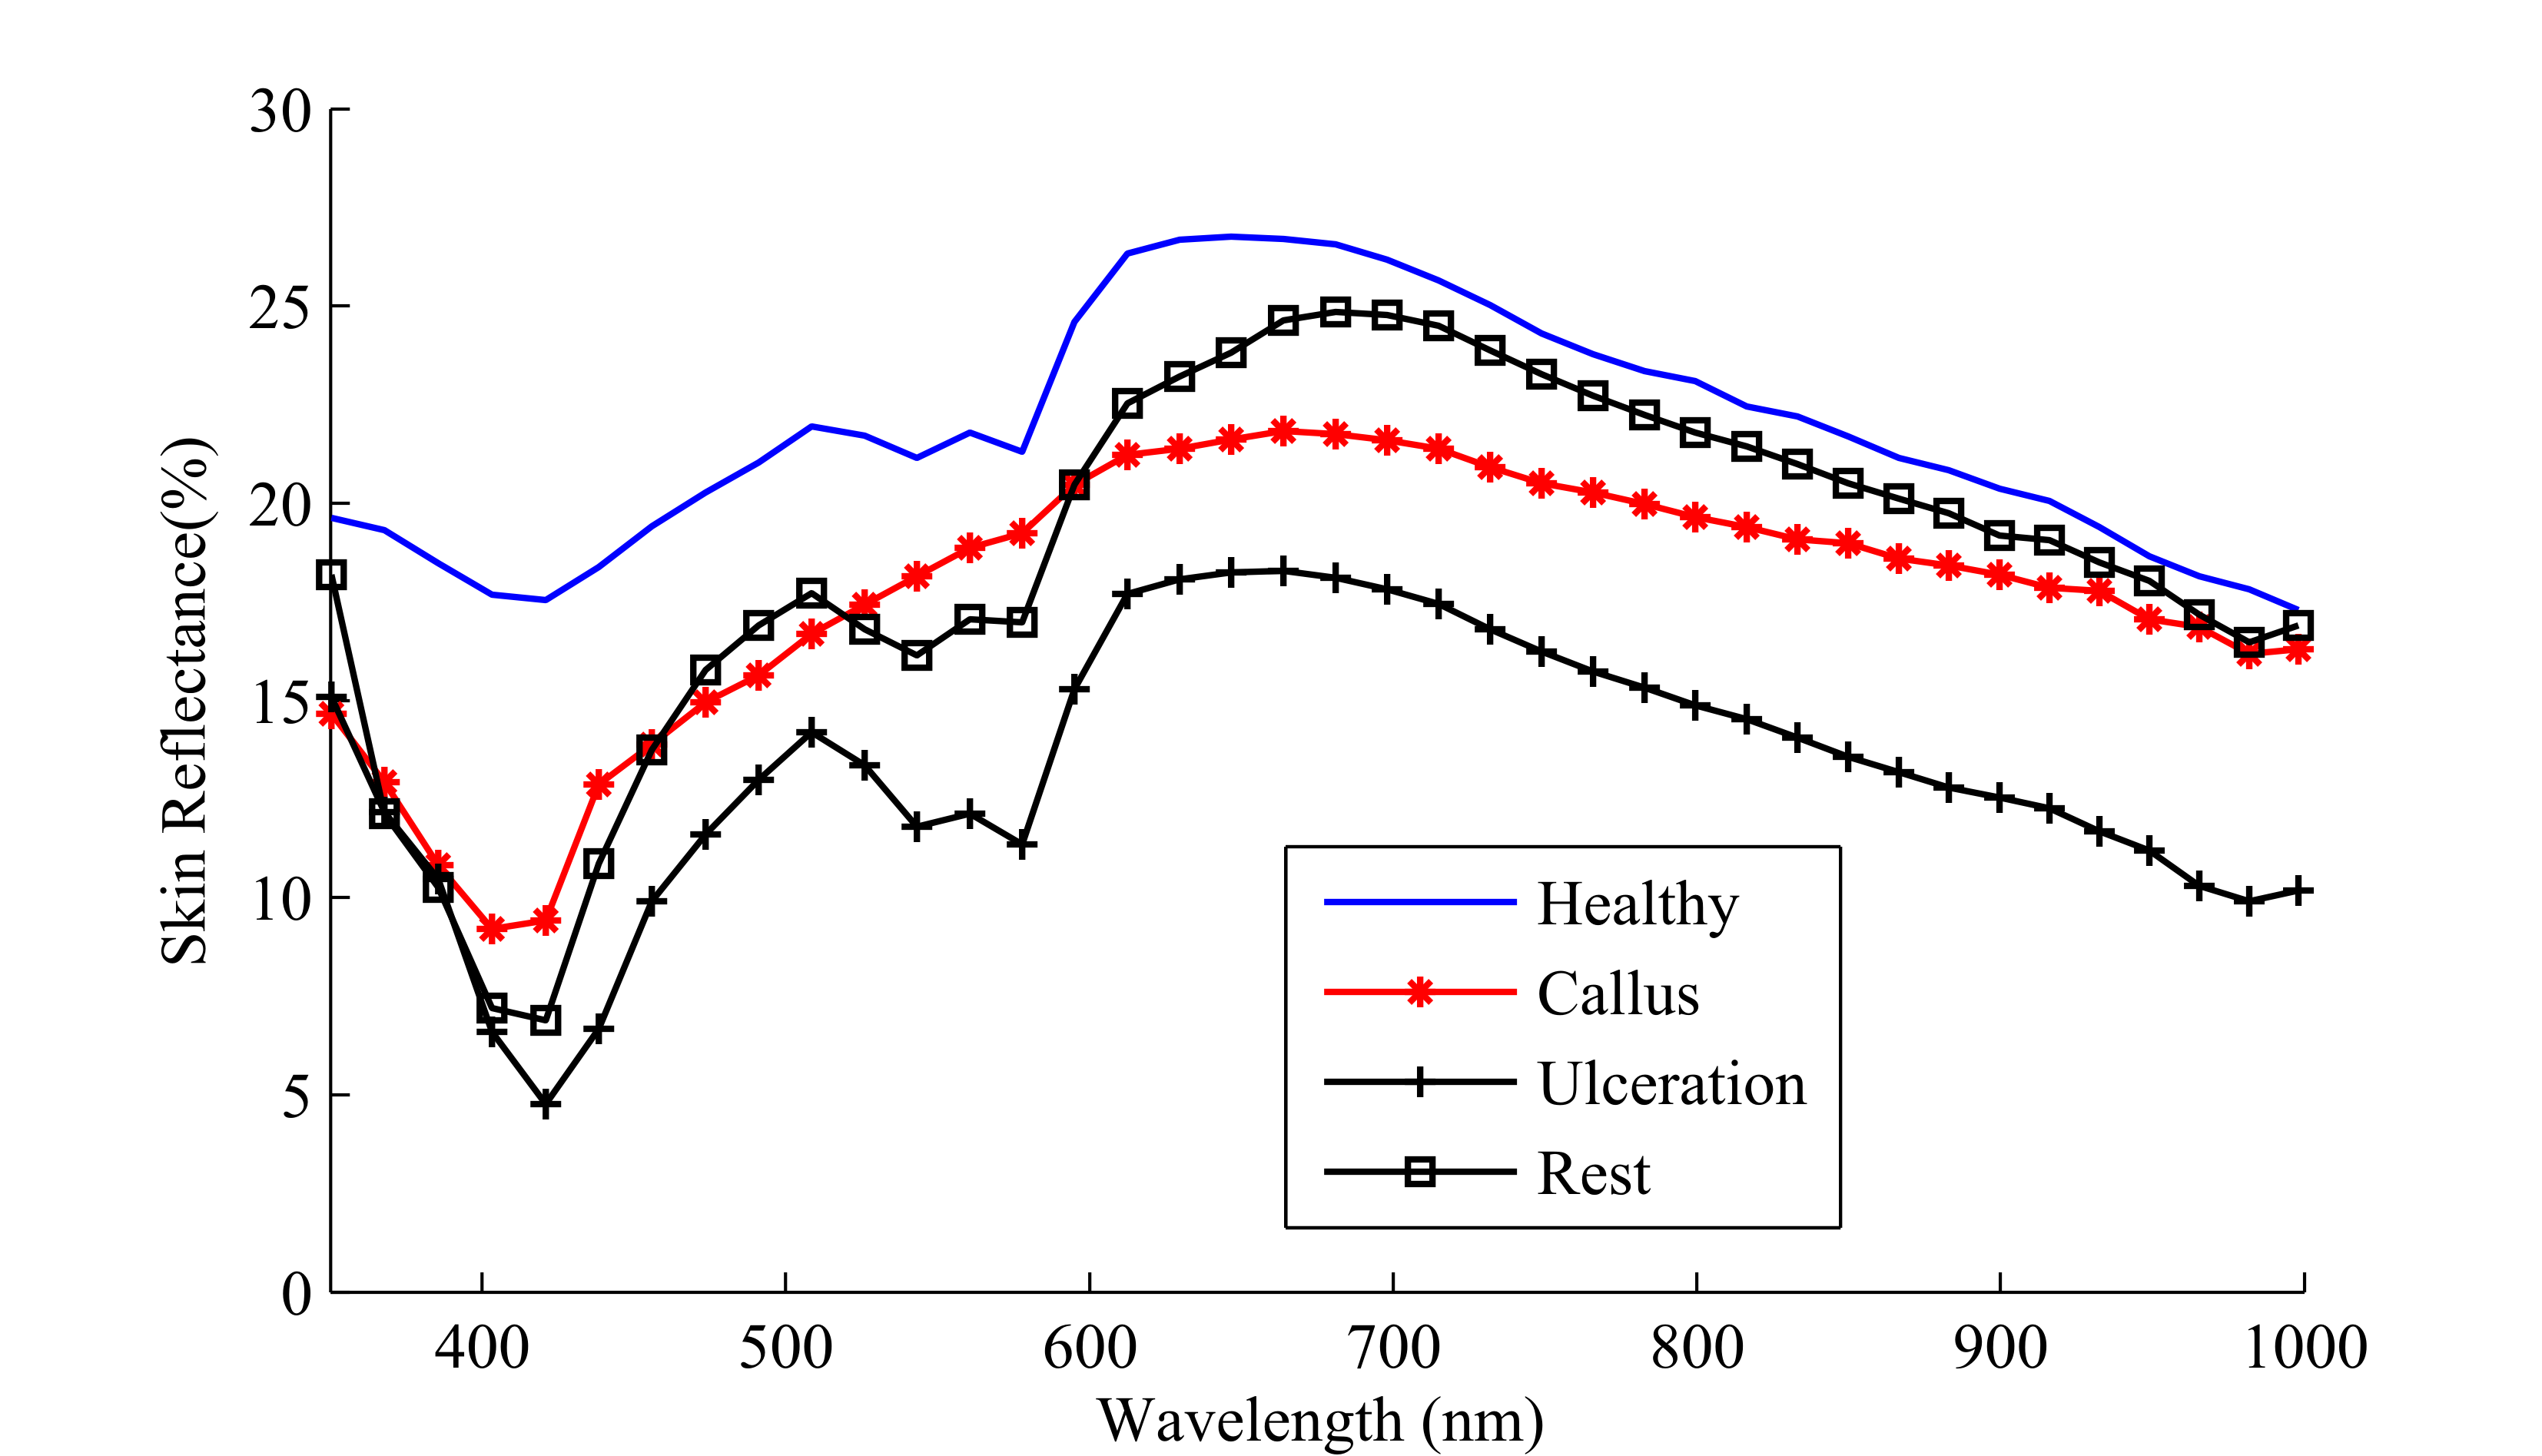
\includegraphics[width=2.5in, height=1.4in]{examples.png}
%         \caption{Examples of spectrum from different classes}
%         \label{fig:example}
% \end{figure}

% Note that IEEE typically puts floats only at the top, even when this
% results in a large percentage of a column being occupied by floats.


% An example of a double column floating figure using two subfigures.
% (The subfig.sty package must be loaded for this to work.)
% The subfigure \label commands are set within each subfloat command, the
% \label for the overall figure must come after \caption.
% \hfil must be used as a separator to get equal spacing.
% The subfigure.sty package works much the same way, except \subfigure is
% used instead of \subfloat.
%
%\begin{figure*}[!t]
%\centerline{\subfloat[Case I]\includegraphics[width=2.5in]{subfigcase1}%
%\label{fig_first_case}}
%\hfil
%\subfloat[Case II]{\includegraphics[width=2.5in]{subfigcase2}%
%\label{fig_second_case}}}
%\caption{Simulation results}
%\label{fig_sim}
%\end{figure*}
%
% Note that often IEEE papers with subfigures do not employ subfigure
% captions (using the optional argument to \subfloat), but instead will
% reference/describe all of them (a), (b), etc., within the main caption.


% An example of a floating table. Note that, for IEEE style tables, the 
% \caption command should come BEFORE the table. Table text will default to
% \footnotesize as IEEE normally uses this smaller font for tables.
% The \label must come after \caption as always.
%
% \begin{table}[!t]
% %% increase table row spacing, adjust to taste
% \renewcommand{\arraystretch}{1.3}
% % if using array.sty, it might be a good idea to tweak the value of
% %\extrarowheight as needed to properly center the text within the cells
% \caption{An Example of a Table}
% \label{table_example}
% \centering
% %% Some packages, such as MDW tools, offer better commands for making tables
% %% than the plain LaTeX2e tabular which is used here.
% \begin{tabular}{|c||c|}
% \hline
% One & Two\\
% \hline
% Three & Four\\
% \hline
% \end{tabular}\label{tab:example}
% \end{table}


% Note that IEEE does not put floats in the very first column - or typically
% anywhere on the first page for that matter. Also, in-text middle ("here")
% positioning is not used. Most IEEE journals use top floats exclusively.
% Note that, LaTeX2e, unlike IEEE journals, places footnotes above bottom
% floats. This can be corrected via the \fnbelowfloat command of the
% stfloats package.









% if have a single appendix:
%\appendix[Proof of the Zonklar Equations]
% or
%\appendix  % for no appendix heading
% do not use \section anymore after \appendix, only \section*
% is possibly needed

% use appendices with more than one appendix
% then use \section to start each appendix
% you must declare a \section before using any
% \subsection or using \label (\appendices by itself
% starts a section numbered zero.)
%



% \section{Matlab script for resizing a video}



% \lstset{language=Matlab,%
% basicstyle=\tiny\ttfamily,
% breaklines=true,%
% morekeywords={matlab2tikz},
% keywordstyle=\color{NavyBlue},%
% morekeywords=[2]{1}, keywordstyle=[2]{\color{black}},
% identifierstyle=\color{black},%
% stringstyle=\color{OrangeRed},
% commentstyle=\color{OliveGreen},%
% showstringspaces=false,%without this there will be a symbol in the places where there is a space
% %numbers=left,%
% %numberstyle={\tiny \color{black}},% size of the numbers
% %numbersep=9pt, % this defines how far the numbers are from the text
% %emph=[1]{for,end,break},emphstyle=[1]\color{red}, %some words to emphasise
% %emph=[2]{word1,word2}, emphstyle=[2]{style}, 
% }

% %\lstinputlisting{convertvideo.m}
% \lstinputlisting[language=Matlab]{convertvideo.m}


% you can choose not to have a title for an appendix
% if you want by leaving the argument blank
% Can use something like this to put references on a page
% by themselves when using endfloat and the captionsoff option.
\ifCLASSOPTIONcaptionsoff
  \newpage
\fi



% trigger a \newpage just before the given reference
% number - used to balance the columns on the last page
% adjust value as needed - may need to be readjusted if
% the document is modified later
%\IEEEtriggeratref{8}
% The "triggered" command can be changed if desired:
%\IEEEtriggercmd{\enlargethispage{-5in}}

% references section

% can use a bibliography generated by BibTeX as a .bbl file
% BibTeX documentation can be easily obtained at:
% http://www.ctan.org/tex-archive/biblio/bibtex/contrib/doc/
% The IEEEtran BibTeX style support page is at:
% http://www.michaelshell.org/tex/ieeetran/bibtex/
%\bibliographystyle{IEEEtran}
% argument is your BibTeX string definitions and bibliography database(s)
%\bibliography{IEEEabrv,../bib/paper}
%
% <OR> manually copy in the resultant .bbl file
% set second argument of \begin to the number of references
% (used to reserve space for the reference number labels box)
\begin{thebibliography}{5}

 \bibitem{KL}
  Lucas, Bruce D., and Takeo Kanade. "An iterative image registration technique with an application to stereo vision." (1981): 674.
\bibitem{KLT}
Tomasi, Carlo, and Takeo Kanade. "Detection and tracking of point features." (1991).
\bibitem{triangulation}
Hartley, Richard, and Andrew Zisserman. Multiple view geometry in computer vision. Cambridge university press, p. 312, 2003.
\bibitem{matlabClass}
Ross Kinard (2020). MultiObjectTrackerKLT, MATLAB Central File Exchange. Retrieved 2020 

(https://www.mathworks.com/matlabcentral/fileexchange/68811-multiobjecttrackerklt).
\end{thebibliography}

% biography section
% 
% If you have an EPS/PDF photo (graphicx package needed) extra braces are
% needed around the contents of the optional argument to biography to prevent
% the LaTeX parser from getting confused when it sees the complicated
% \includegraphics command within an optional argument. (You could create
% your own custom macro containing the \includegraphics command to make things
% simpler here.)
%\begin{biography}[{\includegraphics[width=1in,height=1.25in,clip,keepaspectratio]{mshell}}]{Michael Shell}
% or if you just want to reserve a space for a photo:

%\begin{IEEEbiography}{Michael Shell}
%Biography text here.
%\end{IEEEbiography}

% if you will not have a photo at all:
%\begin{IEEEbiographynophoto}{John Doe}
%Biography text here.
%\end{IEEEbiographynophoto}

% insert where needed to balance the two columns on the last page with
% biographies
%\newpage

%\begin{IEEEbiographynophoto}{Jane Doe}
%Biography text here.
%\end{IEEEbiographynophoto}

% You can push biographies down or up by placing
% a \vfill before or after them. The appropriate
% use of \vfill depends on what kind of text is
% on the last page and whether or not the columns
% are being equalized.

%\vfill

% Can be used to pull up biographies so that the bottom of the last one
% is flush with the other column.
%\enlargethispage{-5in}



% that's all folks
\end{document}


